\documentclass[11pt]{article}
\usepackage[T1]{fontenc}
\usepackage{lmodern}
\usepackage[margin=1.05in]{geometry}
\usepackage{amsmath,amssymb,amsthm,mathtools}
\usepackage{microtype}
\usepackage{enumitem}
\usepackage{booktabs,array}
\usepackage{graphicx}
\usepackage{flafter}
\usepackage{xcolor}
\usepackage{tikz}
\usetikzlibrary{arrows.meta,positioning,calc,decorations.pathreplacing}
\usepackage[numbers,sort&compress]{natbib}
\usepackage[colorlinks=true,linkcolor=blue!45!black,citecolor=blue!45!black,urlcolor=blue!45!black]{hyperref}
\hypersetup{pdftitle={Elementary positivity of chromatic quasisymmetric functions},pdfauthor={OpenAI},pdfsubject={Elementary positivity and terminating permutation witnesses for natural unit interval graphs}}
\numberwithin{equation}{section}
\newtheorem{theorem}{Theorem}[section]
\newtheorem{proposition}[theorem]{Proposition}
\newtheorem{lemma}[theorem]{Lemma}
\newtheorem{corollary}[theorem]{Corollary}
\theoremstyle{definition}
\newtheorem{definition}[theorem]{Definition}
\newtheorem{example}[theorem]{Example}
\theoremstyle{remark}
\newtheorem{remark}[theorem]{Remark}
\newcommand{\N}{\mathbb N}
\newcommand{\Z}{\mathbb Z}
\newcommand{\Q}{\mathbb Q}
\newcommand{\R}{\mathbb R}
\newcommand{\C}{\mathbb C}
\newcommand{\cF}{\mathcal F}
\DeclareMathOperator{\gr}{gr}
\DeclareMathOperator{\Hilb}{Hilb}
\DeclareMathOperator{\Ad}{Ad}
\DeclareMathOperator{\supp}{supp}
\DeclareMathOperator{\id}{id}
\DeclareMathOperator{\Sym}{Sym}
\DeclareMathOperator{\ginv}{ginv}
\DeclareMathOperator{\inv}{inv}
\setlist{itemsep=3pt,topsep=5pt}
\setlength{\emergencystretch}{2em}
\title{Elementary positivity of chromatic\\quasisymmetric functions}
\author{OpenAI}
\date{September 24, 2026}
\begin{document}
\maketitle
\begin{abstract}
We prove that the chromatic quasisymmetric function of every natural unit
interval graph is elementary-positive over $\N[q]$. This resolves the
elementary-positivity part of the Shareshian--Wachs conjecture.
\end{abstract}
\tableofcontents
\section{Introduction}
\label{main:introduction}

Let $h=(h(1),\ldots,h(n))$ be a weakly increasing integer sequence with
$i\le h(i)\le n$. The associated \emph{natural unit interval graph} has
vertex set $[n]=\{1,\ldots,n\}$ and edges
\[
 E(G)=\bigl\{\{i,j\}:i<j\le h(i)\bigr\}.
\]
These are also called naturally labeled Dyck graphs. A proper coloring is a
map $f:[n]\to\N_{>0}$ that has distinct values on adjacent vertices. In the
variable alphabet $X=(x_1,x_2,\ldots)$ put
\begin{equation}
 \chi_G(X;q)=\sum_{f\text{ proper}}
 q^{\operatorname{asc}_G(f)}\prod_{a=1}^n x_{f(a)},
 \qquad
 \operatorname{asc}_G(f)=
 \#\{\{a,b\}\in E(G):a<b,\ f(a)<f(b)\}.
 \label{main:csf}
\end{equation}
Shareshian and Wachs proved that this function is symmetric for this graph
class and conjectured that its coefficients in the elementary basis belong
to $\N[q]$ \cite{SW16}. Here
$e_k(X)=\sum_{i_1<\cdots<i_k}x_{i_1}\cdots x_{i_k}$ and
$e_\lambda=\prod_i e_{\lambda_i}$ for a partition $\lambda$.

The coefficients admit a more precise interpretation in terms of
permutations. Define
\begin{align*}
 D_G^0&=\{\sigma\in S_n:
   \sigma_i>\sigma_{i+1}\Longrightarrow
   \{\sigma_i,\sigma_{i+1}\}\in E(G)\},\\
 \ginv_G(\sigma)&=\#\{(i,j):i<j,\ \sigma_i>\sigma_j,
                    \{\sigma_i,\sigma_j\}\in E(G)\}.
\end{align*}
Thus $D_G^0$ forbids adjacent descents between nonneighbors, and
$\ginv_G$ counts only inversions supported on edges.

\begin{theorem}[Elementary positivity and a permutation witness]
\label{main:theorem}
There is a deterministic terminating procedure which, given a natural
unit interval graph $G$ on $[n]$ and $\sigma\in D_G^0$, returns a partition
$\theta_G(\sigma)\vdash n$ such that
\begin{equation}
 \chi_G(X;q)=\sum_{\sigma\in D_G^0}
       q^{\ginv_G(\sigma)}e_{\theta_G(\sigma)}(X).
 \label{main:witness}
\end{equation}
In particular every elementary coefficient of $\chi_G(X;q)$ belongs to
$\N[q]$. The assertion holds as a formal symmetric-function identity,
uniformly in $n$ and $G$.
\end{theorem}

This proves the elementary-positivity part of the Shareshian--Wachs
conjecture. The theorem makes no assertion of elementary unimodality.
The construction specifies a map on individual inputs: it does not take
the elementary coefficient list as input and redistribute permutations
according to that list. Its running time may nevertheless be large.

For example, let $G$ be the path $1$--$2$--$3$. Its expansion is
\begin{equation}
 \chi_G(X;q)=q\,e_{(2,1)}(X)+(1+q+q^2)e_{(3)}(X).
 \label{main:path-example}
\end{equation}
Write $m_\lambda$ for the sum of the distinct monomials with exponent
multiset $\lambda$. To check this directly, the colorings with a repeated color contribute
$q\,m_{(2,1)}(X)$, while those with three distinct colors contribute
$(1+4q+q^2)m_{(1,1,1)}(X)$. Now use
$e_{(2,1)}=m_{(2,1)}+3m_{(1,1,1)}$ and
$e_{(3)}=m_{(1,1,1)}$.
The domain $D_G^0$ consists of $123,132,213,321$, with graph-inversion
degrees $0,1,1,2$. The theorem assigns one of the two degree-one
permutations to $(2,1)$ and the other three permutations to $(3)$.
Thus the map refines the degree count by an entire elementary partition.
Equation~\eqref{main:path-example} alone does not specify which of
$132$ and $213$ receives which partition; the procedure in
Section~\ref{route:section} makes that individual choice.

The positivity question is difficult because the coloring definition
already has nonnegative coefficients in the monomial variables, whereas
rewriting it in the elementary basis can involve subtraction.  Our proof
separates this issue from the individual assignment.  It first identifies
each relevant elementary coefficient with a positive algebraic object.
It then realizes the algebraic identities by finite bijections between
ordered collections of independent sets. Neither stage uses the sought elementary
coefficient list as input to the permutation rule.

\subsection{History and significance}

The problem grew out of positivity questions for immanants of
Jacobi--Trudi matrices, studied by Haiman and by Stanley and Stembridge
\cite{Hai93,SS93}.  Stanley introduced the chromatic symmetric function
as a symmetric-function refinement of the chromatic polynomial
\cite{Sta95}; it is the specialization of
Equation~\eqref{main:csf} at $q=1$.  In this language, the
Stanley--Stembridge conjecture asks for elementary positivity of the
incomparability graphs of $(3+1)$-free posets
\cite[Conjecture~5.5]{SS93}. The incomparability graph joins two
elements exactly when neither is below the other. A poset is
$(3+1)$-free if it has no induced three-element chain together with
an element incomparable to that chain.
Guay-Paquet's reduction expresses its chromatic symmetric function as
a nonnegative rational combination of those of unit interval orders
\cite[Theorem~5.1]{GP13}. Their naturally labeled incomparability
graphs are the graphs in Theorem~\ref{main:theorem}. Specializing our
theorem at $q=1$ therefore also proves the classical positivity
theorem, previously established by Hikita \cite{Hik24}.

Positive expansions in other bases provided important earlier
structure. Haiman's immanant results imply Schur positivity for
incomparability graphs of $(3+1)$-free posets \cite{Hai93}; Gasharov
gave a positive formula using poset tableaux \cite{Gas96}. Chow's
quasisymmetric expansion related chromatic symmetric functions to
permutation descents \cite{Cho99}.  Shareshian and Wachs introduced the
$q$-refinement in Equation~\eqref{main:csf}, proved its symmetry and
Schur positivity for natural unit interval graphs, and formulated the
elementary-positivity and elementary-unimodality conjecture
\cite{SW12,SW16}.  Their acyclic-orientation formula gives elementary
coefficients after grouping partitions by their number of parts
\cite[Theorem~5.3]{SW16}; Athanasiadis supplied a power-sum expansion
\cite{Ath15}.  These descriptions do not determine a nonnegative
coefficient formula for each elementary partition.

The geometric connection gives another reason to study the
$q$-grading.  Tymoczko constructed permutation actions on equivariant
cohomology \cite{Tym08}, and Shareshian and Wachs related their
chromatic functions conjecturally to the graded representation on
regular semisimple Hessenberg varieties \cite{SW12,SW16}.
Brosnan--Chow and Guay-Paquet proved this representation-theoretic
identity \cite{BC18,GP16}.  That result is distinct from the
elementary-positivity assertion addressed here.  Geometric,
combinatorial and algebraic approaches subsequently established
positivity for substantial families: abelian Hessenberg varieties
\cite{HP19}, classes treated by explicit elementary expansions
\cite{CH19}, melting lollipops \cite{HNY20}, and the $q$-rook
formulas for abelian Dyck paths \cite{CMP23}.  The modular law also
provided a systematic tool for organizing chromatic functions and
their relations \cite{AN21}.

Hikita's proof uses a probabilistic formula \cite{Hik24}. His formula gives numerical
nonnegativity for every positive real $q$, while its rational
$q$-weights do not establish coefficientwise nonnegativity in $\N[q]$;
the refined conjecture remains explicitly distinguished in
\cite[Section~1.3]{Hik24}.  Griffin, Mellit, Romero, Weigl and Wen gave
an independent proof through Macdonald expansions, recovering Hikita's
elementary formula \cite{GMRWW25}. Further developments include
positivity at $q=1$ of the Abreu--Nigro $g$-functions, proved by
Huh, Hwang, Kim, Kim and Oh as a refinement of Hikita's theorem
\cite{HHKKO25},
Chow's combinatorial interpretation of the probabilities \cite{Chow26},
and lower bounds for elementary coefficients studied by Siegl
\cite{Siegl26}.  Theorem~\ref{main:theorem} gives a formal polynomial
formula with nonnegative integer coefficients and an individual
assignment preserving the specified graph-inversion weight.

The representation identity and Theorem~\ref{main:theorem} give the
following degreewise consequence.

\begin{corollary}[Young permutation modules in Hessenberg cohomology]
\label{main:hessenberg}
Let $n\ge1$, let $h$ be as above with graph $G=G(h)$, and let
$S\in M_n(\C)$ be regular semisimple. Write
\[
 \operatorname{Hess}(S,h)=
 \{F_\bullet\in\operatorname{Flag}(\C^n):
     SF_i\subseteq F_{h(i)}\text{ for all }i\}.
\]
For $\lambda=(\lambda_1,\ldots,\lambda_\ell)\vdash n$, let
$M^\lambda=\operatorname{Ind}_{S_\lambda}^{S_n}\mathbf{1}_{\C}$ be the
Young permutation module, where
$S_\lambda=S_{\lambda_1}\times\cdots\times S_{\lambda_\ell}$ is the
standard Young subgroup, and put
\[
 m_{\lambda,d}(h)=
 \#\{\sigma\in D_G^0:\theta_G(\sigma)=\lambda,\ \ginv_G(\sigma)=d\}.
\]
Then for every integer $d\ge0$, under Tymoczko's dot action on ordinary
cohomology there is an abstract $\C[S_n]$-module isomorphism
\[
 H^{2d}(\operatorname{Hess}(S,h);\C)
 \cong\bigoplus_{\lambda\vdash n}(M^\lambda)^{\oplus m_{\lambda,d}(h)}.
\]
\end{corollary}

\begin{proof}
Write $\operatorname{ch}$ for the Frobenius characteristic and $\omega$
for the usual symmetric-function involution, so
$\omega(e_\lambda)=h_\lambda$, the product of complete homogeneous
symmetric functions. The identity of Brosnan--Chow
\cite[Theorem~129]{BC18} and Guay-Paquet \cite{GP16}, followed by
Equation~\eqref{main:witness}, gives
\[
 \operatorname{ch}H^{2d}(\operatorname{Hess}(S,h);\C)
 =[q^d]\,\omega\chi_G(X;q)
 =\sum_{\lambda\vdash n}m_{\lambda,d}(h)h_\lambda.
\]
Since $\operatorname{ch}M^\lambda=h_\lambda$
\cite[proof of Proposition~10]{BC18}, injectivity of the Frobenius
characteristic and complete reducibility of finite-dimensional complex
$S_n$-modules give the isomorphism.
The argument supplies no preferred isomorphism, geometric basis, or
compatibility with cup product.
\end{proof}

There is also a direct precedent for asking for a partition-valued
permutation rule.  Stanley and Stembridge proposed such an assignment
on their compatible permutations \cite[Remark~5.6]{SS93}.  That proposal
concerns the ungraded elementary expansion.  The rule here retains the
full graph-inversion degree and specifies a terminating procedure on
each input.  The finite cancellation used to pass from required
ascents to exact ascents belongs to the bijective-cancellation
tradition represented by the Garsia--Milne involution principle
\cite{GM81}.

Our algebraic reduction likewise has substantial antecedents.
Stanley's graph specialization \cite[Section~2]{Sta98}, chromatic functions in
noncommuting variables \cite{GS01}, and the noncommutative
symmetric-function methods of Fomin--Greene and Blasiak--Fomin
\cite{FG98,BF17} provide a framework for commuting symmetric expressions
inside a noncommutative algebra.  Hwang's noncommutative
$P$-symmetric functions \cite{Hwa24} and the poset algebras of Blasiak,
Eriksson, Pylyavskyy and Siegl \cite{BEPS25} provide direct predecessors
of the graph-alphabet evaluation and its elementary/monomial
coefficient pairing.  We give a short proof in the centered quantum
torus conventions needed for the subsequent argument.

The positive factorization and transport stages use the mathematical
framework of Hall algebras and scattering diagrams.  Ordered slope
factorization and polynomial shuffle products were developed in
\cite{Rei03,KS11}, with semistable quotient and integrality results in
\cite{Ef12,FR18,DMe20}.  The connection from Hall factorization to
wall transformations appears in Reineke's Poisson automorphisms and
Bridgeland's stability scattering diagrams \cite{Rei10,Bri17}.
Scattering constructions originate in work of Kontsevich--Soibelman
and Gross--Siebert \cite{KS06,GS11,KS14}; theta bases and mutation are
central to the cluster framework of Gross--Hacking--Keel--Kontsevich
\cite{GHKK18}, and Davison--Mandel prove strong quantum positivity
\cite{DM21}.  We prove the particular reordering, completion and
transport statements needed here with their explicit gradings and
finite coefficient bounds.  The graph-specific step is then an
identification: general positivity of theta sections does not itself
show that a graph-alphabet monomial symmetric function is one such
section.  The triangular chart below proves that identity before the
packet construction extracts the individual witness.

\subsection{Proof structure}

The first reduction replaces colorings by coefficients in an algebra
whose monomials record vertex multiplicities. Write $q=v^2$ and let
$X_m$ denote the basis monomial indexed by a vertex-multiplicity
vector $m$.  Multiplication of these monomials is
twisted by an alternating form recording ordered edges. For a larger unit
interval graph $\Gamma$ containing $G$, let $E_k$ be the sum of the
monomials of independent $k$-sets. We prove that the $E_k$ commute, so
they may be evaluated as elementary symmetric functions $e_k(Y)$ of a
formal alphabet $Y$. If $u$ is the sum of the original vertex exponents
and $M=|E(G)|$, the elementary coefficient becomes
\begin{equation}
 [e_\lambda(X)]\chi_G(X;v^2)
       =v^M[X_u]m_\lambda(Y).
 \label{main:reduction}
\end{equation}
Here $m_\lambda$ is the monomial symmetric function. The identity is
proved in Proposition~\ref{graph:kernel}.

The central step is to identify $m_\lambda(Y)$ as a chamber value of a
single positive section of a system of wall transformations. A wall is
a portion of a hyperplane in the real dual of the exponent lattice,
equipped with conjugation by a formal series. A section is a family of
chamber values related by these transformations. We construct sections $\Theta_m$,
indexed by lattice exponents, by prescribing their coefficients in test
directions determined by the alternating form. The auxiliary graph is
arranged in a triangle with distinguished independent vertices
$d_1,\ldots,d_D$, called anchors. For a partition $\lambda$ of length
at most $D$, padded by zeroes to length $D$, the essential identification in the all-negative chamber is
\begin{equation}
 m_\lambda(Y)=\Theta_{\lambda_1d_1+\cdots+\lambda_Dd_D}.
 \label{main:identification}
\end{equation}
Repeated interval rotations establish this identity. A support argument
using positive powers of $E_1$ is essential: stationarity under the
rotations alone does not force an exponent to involve anchors only.

The proof has three main components.  First, positive quantum factors
remain positive when their order is reversed.  We realize the new
multiplicities as dimensions of explicit graded vector spaces, and
prove the coefficient bounds needed for all infinite series.
Second, the interval rotations identify a family of graph symmetric
functions with single positive theta sections. Together with
Equation~\eqref{main:reduction}, this already proves coefficientwise
elementary positivity. Third, we extract the individual assignment.
After reversing an input permutation, we group vertices into packets,
each an independent set written in increasing order. A local packet
bijection transports them to subsets of the independent anchors and
records weighted jumps. The total jump histories are independent of
packet sizes. Finite matching cancellation refines required nonedge
ascents of input words and required strict ascents of anchor words to
exact sets of such positions. The empty set on the anchor side leaves
a weakly decreasing word, whose multiplicities give the output partition. The finite
matching argument supplies termination without consulting the desired
final shape counts.

Section~\ref{graph:section} proves the coloring reduction and fixes
permutation conventions. Section~\ref{alg:section} proves the
reordering result. Section~\ref{wall:section} constructs the wall
sections and proves their positivity and mutation rules.
Section~\ref{tri:section} establishes
Equation~\eqref{main:identification}, and
Section~\ref{route:section} constructs the individual permutation map.
Section~\ref{main:completion} returns to the original graph and proves
Theorem~\ref{main:theorem}, including the reversal needed for the
convention in $D_G^0$.

\section{Graph alphabets and the coloring reduction}
\label{graph:section}

This section reduces the elementary expansion to coefficients of
monomial symmetric functions evaluated in a quantum torus. It also
fixes the permutation convention used by the transport construction.

\subsection{Admissible words and insertion digits}

For the graph $G$ in the introduction put
$l_a=\#\{b<a:\{b,a\}\in E(G)\}$ and $M=\sum_a l_a$.
The earlier neighbors of $a$ are a suffix of $[a-1]$, and they form a
clique. Let
\[
 \mathcal A_G=\{w\in S_n:
    w_i<w_{i+1}\Longrightarrow\{w_i,w_{i+1}\}\in E(G)\}.
\]
We call these words \emph{admissible}. Their forbidden adjacent pairs
are nonedge ascents. Write $\inv_G(w)$ for their edge-inversion count,
given by the same formula as $\ginv_G$.

\begin{lemma}[Insertion digits]
\label{graph:digits}
There is a bijection between $\mathcal A_G$ and the sequences
$(j_1,\ldots,j_n)$ with $0\le j_a\le l_a$. Under this bijection,
$\inv_G(w)=\sum_a j_a$. Reversal is a bijection
$D_G^0\to\mathcal A_G$, and
\begin{equation}
 \inv_G(\operatorname{reverse}\sigma)=M-\ginv_G(\sigma).
 \label{graph:reverse}
\end{equation}
\end{lemma}

\begin{proof}
Delete the largest letter $a$ from an admissible word on $[a]$.
If it has predecessor $b$ and successor $c$, then $b<a$ and
$h(b)\ge a>c$, so the newly consecutive pair $(b,c)$ is allowed.
The cases without a predecessor or successor are immediate. Conversely,
$a$ can be inserted at the beginning or immediately after any earlier
neighbor, and these are exactly the allowed positions. At such a
position the new inversions are the earlier neighbors lying to its
right. Reading those neighbors in their order in the shorter word
shows that the available counts are $l_a,l_a-1,\ldots,0$, each once.
Successive insertion and deletion prove the bijection and degree
formula. Reversal exchanges nonedge descents and nonedge ascents and
reverses the order of the endpoints of every edge, proving
Equation~\eqref{graph:reverse}.
\end{proof}

The relation $a<b$ and $\{a,b\}\notin E(G)$ is transitive: it is
equivalent to $h(a)<b$. Consequently, an increasing word in which each
adjacent pair is a nonedge lists an independent set. This observation
will identify packets of independent vertices with required ascent
positions in Section~\ref{route:section}.

\subsection{The quantum torus of an ordered graph}

For this subsection let $\Gamma$ be any natural unit interval graph on
a finite ordered vertex set. Let $L_\Gamma$ be the free abelian group
on its vertices, identifying a vertex with its basis vector. Define an
integer alternating form by
\begin{equation}
 \Omega(b,a)=
 \begin{cases}1,&a<b\text{ and }\{a,b\}\in E(\Gamma),\\
                0,&a<b\text{ and }\{a,b\}\notin E(\Gamma),
 \end{cases}
 \label{graph:form}
\end{equation}
and extend by bilinearity and skew symmetry. Over
$\Q((v^{-1}))$, the quantum torus has basis $X_m$, $m\in L_\Gamma$,
and product
\begin{equation}
 X_mX_{m'}=v^{\Omega(m,m')}X_{m+m'}.
 \label{graph:torus}
\end{equation}
The coefficient field consists of Laurent series with bounded upper
powers of $v$. All elements considered in this section are finite
Laurent polynomials; the additional cone completions will be specified
when needed.

For a set $I$ of vertices write $a_I=\sum_{a\in I}a$, and define
\begin{equation}
 E_k(\Gamma)=\sum_{\substack{I\subseteq V(\Gamma)\text{ independent}\\|I|=k}}
 X_{a_I},\qquad E_0(\Gamma)=1.
 \label{graph:elementaries}
\end{equation}

The graph alphabet used here is a centered quantum-torus version of
noncommutative poset symmetric functions \cite{Hwa24,BEPS25}.  More
precisely, on $V(\Gamma)$ define $a<_P b$ when $a<b$ and $\{a,b\}$ is a nonedge.
The chain elementary sums in \cite[Equation~(2.4)]{BEPS25} become our
independent-set sums, and the relations in
\cite[Definition~3.16]{BEPS25} become the relations above under
$u_a\mapsto X_a$ and $t\mapsto v^2$.  We prove commutation directly
in these conventions.

\begin{proposition}[Commuting independent-set sums]
\label{graph:commutation}
For every natural unit interval graph $\Gamma$ and all $j,k\ge0$,
$E_j(\Gamma)E_k(\Gamma)=E_k(\Gamma)E_j(\Gamma)$.
\end{proposition}

\begin{proof}
We adapt the two-color involution underlying
\cite[Lemma~4.4 and Theorem~4.5]{SW16}.
A term on the left is an ordered pair of independent sets $(I,J)$,
with exponent $a_I+a_J$ and weight $v^{\Omega(a_I,a_J)}$.
Vertices in $I\cap J$ have no neighbors in $I\cup J$ and contribute
no skew weight. In the remaining induced graph, every earlier-neighbor
set and every later-neighbor set is a clique. Since the graph is
bipartite with parts $I\setminus J$ and $J\setminus I$, each vertex
has at most one earlier and one later neighbor. More explicitly, an
edge that skipped a vertex of $I\cup J$ in the total order would make
a triangle: the interval-closure property supplies both intervening
edges. Thus each nontrivial component is an increasing path with
alternating membership in $I$ and $J$.

On every component with an odd number of vertices, exchange the two
memberships; keep the even components and the doubled isolated
vertices unchanged. Every even component has equally many vertices in
the two sets. Every odd component reverses its size difference, so the
new ordered pair $(I',J')$ has sizes $k,j$. On an odd component the
successive edge contributions to $\Omega(a_I,a_J)$ alternate between
$1$ and $-1$, with equally many of each. Its skew contribution is
therefore zero before and after the exchange. There are no edges
between components. Exponents and weights are preserved, and repeating
the exchanges recovers $(I,J)$. This is the required bijection of
terms.
\end{proof}

Let $\alpha(\Gamma)$ denote the maximum size of an independent set in
$\Gamma$, and suppose $\alpha(\Gamma)\le D$. The ring of symmetric polynomials in
$D$ commuting variables is the polynomial ring in $e_1,\ldots,e_D$.
Proposition~\ref{graph:commutation} therefore defines an algebra
homomorphism by $e_k\mapsto E_k(\Gamma)$, with $E_k=0$ for $k>D$.
We denote its value on a symmetric polynomial $F$ by $F(Y)$, and
write $e_k(Y)=E_k$. The symbol $Y$ denotes this evaluation; no
individual roots $y_i$ in the quantum torus are being asserted.
In particular, $m_\lambda(Y)$ is well defined for partitions of length
at most $D$, where $m_\lambda$ is the sum of distinct monomials with
exponent multiset $\lambda$.

\subsection{The elementary coefficient identity}

Let $G$ be the induced ordered graph on distinct vertices
$a_1,\ldots,a_n$ of $\Gamma$, and put $u=a_1+\cdots+a_n$.
For a proper coloring $f$ define
$\operatorname{inv}_G(f)=\#\{a<b:\{a,b\}\in E(G),\ f(a)>f(b)\}$
and let $X_G(X;q)$ be the corresponding proper-color inversion
generating function.

The following coefficient reduction is the elementary/monomial form
of the noncommutative Cauchy pairing in
\cite[Theorem~4.4, Corollary~4.5 and Proposition~4.25]{Hwa24} and
\cite[Proposition~2.9 and Corollary~2.10]{BEPS25}.  We include its
proof to fix the graph-inversion and centered-monomial factors.

\begin{proposition}[Coloring kernel]
\label{graph:kernel}
If $\alpha(\Gamma)\le D$, then $X_G(X;q)$ is symmetric and
\begin{equation}
 X_G(X;v^2)=\sum_{\substack{\lambda\vdash n\\\ell(\lambda)\le D}}
       v^M[X_u]m_\lambda(Y)\,e_\lambda(X).
 \label{graph:coefficient}
\end{equation}
The equality is independent of the extra vertices of $\Gamma$.
\end{proposition}

\begin{proof}
Work first with $r$ colors. Expand the product, in increasing color
order,
\[
 \prod_{c=1}^r\left(\sum_{k=0}^D x_c^k E_k\right).
\]
Its $X_u$ coefficient chooses a disjoint independent set for each
color, covering precisely the original vertices. Extra vertices
cannot occur because each exponent in each factor has nonnegative
vertex coordinates. These choices are exactly the proper colorings.
An edge whose later vertex has smaller color contributes $+1$ to the
torus exponent, and an edge whose earlier vertex has smaller color
contributes $-1$. The total exponent is
$2\operatorname{inv}_G(f)-M$. Hence multiplying this coefficient by
$v^M$ gives $X_G(x_1,\ldots,x_r;v^2)$.

For ordinary variables $y_1,\ldots,y_D$ the elementary dual kernel
identity is
\[
 \prod_{c=1}^r\prod_{i=1}^D(1+x_cy_i)
   =\sum_\lambda e_\lambda(x_1,\ldots,x_r)m_\lambda(y_1,\ldots,y_D).
\]
Indeed, select for each labeled $y_i$ a subset of the $x$ variables;
grouping its subset sizes by their multiset gives the displayed sum.
Evaluate the symmetric $y$ polynomials at $Y$, extract $X_u$, and
multiply by $v^M$. This proves Equation~\eqref{graph:coefficient} for
every $r$, and therefore as a symmetric-function identity. The
coloring interpretation proves independence of the ambient graph.
\end{proof}

\begin{example}[The centered normalization on two vertices]
Let $\Gamma=G$ have ordered vertices $a<b$. If they are adjacent,
$E_2=0$ and $m_{(2)}(Y)=E_1^2$ has $X_{a+b}$-coefficient
$v+v^{-1}$. The factor $v^M=v$ in
Equation~\eqref{graph:coefficient} therefore gives
$X_G(X;q)=(1+q)e_2(X)$.
If they are nonadjacent, $E_2=X_{a+b}$ and the two terms in
$E_1^2$ at this exponent each have weight one. Hence
$[X_{a+b}]m_{(2)}(Y)=[X_{a+b}](E_1^2-2E_2)=0$, whereas
$[X_{a+b}]m_{(1,1)}(Y)=[X_{a+b}]E_2=1$, giving
$X_G(X;q)=e_1(X)^2$. Even in this small case, evaluating a monomial
symmetric function requires subtraction; positivity of the generators
$E_k$ by itself does not settle the elementary coefficients.
\end{example}

\begin{lemma}[Color reversal and shape reciprocity]
\label{graph:reciprocity}
For every natural unit interval graph $G$, $X_G(X;q)=\chi_G(X;q)$.
Writing $c_\lambda(q)=[e_\lambda]X_G(X;q)$, one has
\begin{equation}
 c_\lambda(q)=q^M c_\lambda(q^{-1})
 \label{graph:reciprocity-eq}
\end{equation}
for every partition $\lambda$.
\end{lemma}

\begin{proof}
Use $r$ colors and send $f$ to $r+1-f$. This interchanges color
ascents and inversions and reverses the variable alphabet. Symmetry,
which follows from Proposition~\ref{graph:kernel} with
$\Gamma=G$, removes the variable reversal and gives
$X_G=\chi_G$. Since a proper coloring has
$\operatorname{asc}_G(f)+\operatorname{inv}_G(f)=M$, the same
argument gives $X_G(X;q)=q^M X_G(X;q^{-1})$. Take $r\ge n$, so
the elementary functions of degree $n$ are independent, and compare
their coefficients. Passing to the symmetric-function limit proves
Equation~\eqref{graph:reciprocity-eq}.
\end{proof}

It now suffices to prove positivity of
$[X_u]m_\lambda(Y)$ for a suitable ambient graph. The graph used in
Section~\ref{tri:section} has $D$ independent anchors and lies in an
interval of length $D-1$; independent vertices are spaced by at least
one, so its independence number is $D$.
Lemma~\ref{tri:embedding} places every original graph among its
vertices. The next two sections develop the positive wall sections
with which these monomial symmetric functions will be identified.

\section{Positive reordering in a quantum torus}
\label{alg:section}

We prove the algebraic statement that supplies positivity at a wall joint.
The proof keeps two gradings distinct: polynomial degree records powers of
$v$, whereas an auxiliary filtration makes a coproduct regular.  The
resulting algebra need not be commutative.  Its graded vector-space
dimensions nevertheless have the required symmetric-algebra form.

Let $\Gamma$ be a lattice with an integral alternating form $\Omega$, and
let $C\subset\Gamma$ be an additive monoid contained in a strictly convex
cone in a real two-dimensional subspace.  Fix an additive charge
$c:C\to\N$ that is positive away from zero, and assume that
$\{p\in C:c(p)\le B\}$ is finite for every $B$.  The completed quantum
torus has multiplication
\begin{equation}\label{alg:torus}
 X_pX_q=v^{\Omega(p,q)}X_{p+q}
\end{equation}
and coefficients in $\Q((v^{-1}))$.  Thus a coefficient has a bounded
upper $v$-degree and can have infinitely many negative degrees.
For $p\in C\setminus\{0\}$ and $k\in\Z$, define
\begin{equation}\label{alg:units}
 E_{p,k}=\prod_{j\ge0}(1+v^{k-2j}X_p),\qquad
 H_{p,k}=\prod_{j\ge0}(1-v^{k-2j}X_p)^{-1}.
\end{equation}
We call these \emph{elementary units}.  A list of their occurrences is
\emph{admissible} if, for each charge bound $B$, their parameters $k$ are
bounded above and only finitely many occurrences with $c(p)\le B$ have
$k\ge L$, for each $L\in\Z$.  Occurrences are counted with multiplicity.

\begin{theorem}[Positive reordering]\label{alg:reordering}
Suppose an admissible product of elementary units is written in ray
order, with $\Omega(p_i,p_j)>0$ whenever the ray of $p_i$ precedes the
distinct ray of $p_j$.  Its factorization in the opposite ray order is
again a product of elementary units, with nonnegative integral
multiplicities.  The output list is admissible.

Every coefficient at fixed exponent and fixed $v$-degree is a finite
sum of nonnegative integers, and each exponent has bounded upper
$v$-degree.  The assertion also holds modulo any fixed charge cutoff.
For the algorithmic assertion, assume that lattice operations, the form
$\Omega$ and the charge are effectively computable, that input occurrences
at bounded charge and above a given parameter threshold can be listed
effectively, and that for every $B$ one can compute an integer $A_B\ge1$
such that
\[
 |\Omega(p,q)|\le A_B
 \qquad\text{whenever }p,q\in C,\quad c(p),c(q)\le B.
\]
Then every prescribed coefficient and every bounded part of the output
unit list can be calculated by finite rational linear algebra.
\end{theorem}

We first decompose shuffle spaces by slope and use separated-center
restrictions to construct a coproduct on an auxiliary associated graded
space. Polynomiality of the restriction symbols removes negative
separation powers before evaluation at zero. A signed vector-space PBW
decomposition and primitive strings then give the positive elementary
factors. Throughout, polynomial degree with its shifts records powers of
$v$; the final energy bounds control infinite input lists.

A ray factorization with constant term one exists uniquely over
$\Q((v^{-1}))$: at charge $B$, subtract the contributions already
determined at smaller charges, and assign the remaining coefficient of
$X_p$ to the ray of $p$.  Products involving that new coefficient and a
nonconstant term have larger charge.  We shall prove that, in the order
specified in Theorem~\ref{alg:reordering}, each resulting ray factor
has the stronger form asserted there.

\subsection{Shuffle spaces and destabilizing quotients}

Begin with finitely many input occurrences, indexed by $1,\ldots,t$ in
input ray order.  Units on one ray may be ordered arbitrarily.  Set
$a_{ii}=0$ for $E_{p_i,k_i}$ and $a_{ii}=1$ for $H_{p_i,k_i}$.  For
$i\ne j$, put
\[
 a_{ji}=\max\{\Omega(p_i,p_j),0\}.
\]
For dimension vectors $d,e\in\N^t$, define
\begin{align}
 p(d)&=\sum_i d_ip_i,&
 \chi(d,e)&=\sum_i d_ie_i-\sum_{i,j}a_{ij}d_ie_j,
 \label{alg:euler}\\
 s(d)&=\tfrac12\chi(d,d),&
 u(d)&=\sum_i d_i(k_i+1-a_{ii}).
 \label{alg:shifts}
\end{align}
Then
\begin{equation}\label{alg:skew}
 \chi(d,e)-\chi(e,d)=\Omega(p(d),p(e)).
\end{equation}
Choose a linear functional $\eta$ on the plane so that
$\mu(d)=\eta(p(d))/c(p(d))$ increases in input ray order.
This is possible by intersecting the strictly convex cone with
$c=1$.  Dimension vectors of a common slope have symmetric pairings
under $\chi$.  We use $|d|_1=\sum_i d_i$ only to count variables and to
perform inductions; it is different from charge.

Let
\[
 S_d=\Q[x_{i,\alpha}:1\le i\le t,\ 1\le\alpha\le d_i]
       ^{\prod_i\mathfrak S_{d_i}},\qquad S_0=\Q,
\]
with every variable of polynomial degree one.  Variables with a fixed
$i$ form a pack.  The polynomial shuffle presentation is the cohomological Hall product
of Kontsevich--Soibelman \cite[Section~2.4, Theorem~2]{KS11}; see also
\cite[Theorem~2.2]{Ef12}.  In our normalization it is
\begin{equation}\label{alg:shuffle}
 f*g=\sum_{\text{pack shuffles}}f(x)g(y)K_{d,e}(x,y),\qquad
 K_{d,e}(x,y)=
 \prod_{i,j}\prod_{\alpha\le d_i,\,\beta\le e_j}
 (y_{j,\beta}-x_{i,\alpha})^{a_{ij}-\boldsymbol1_{i=j}}.
\end{equation}
Each shuffle chooses, in each output pack, the variables assigned to
the first input; there is no factorial normalization.  The only
possible poles are simple poles between two variables of the same
output pack.  Interchanging those two variables pairs the residues
with opposite signs.  After taking a common denominator, the
numerator is therefore divisible by every such difference.  The
differences are relatively prime irreducible polynomials, so all poles
cancel.  Consequently $f*g\in S_{d+e}$.  A simultaneous shuffle of
three input groups proves associativity: each pair of groups
contributes exactly one kernel in either parenthesization.  Polynomial
degree changes by $-\chi(d,e)$.

The destabilizing quotient below is the polynomial form of the
semistable restriction quotient in \cite[Theorem~8.1]{FR18}.  We
establish its needed properties directly for our charge-weighted slope.
For $d\ne0$, put
\begin{equation}\label{alg:quotient}
 I_d=\sum_{\substack{a+b=d,\ a,b\ne0\\\mu(a)>\mu(d)}}S_a*S_b,
 \qquad B_d=S_d/I_d,
 \qquad B_0=\Q.
\end{equation}
Every image $S_a*S_b$ is an ordinary $S_d$-submodule.  Indeed an
output symmetric polynomial, restricted to the two input packs, is a
finite sum of polynomial tensors; multiplication by it can be moved
inside the shuffle.  Thus $I_d$ is an ordinary homogeneous ideal.

The product descends to $B_d\otimes B_e\to B_{d+e}$ when
$\mu(d)=\mu(e)=\theta$.  If $a+b=d$ and $\mu(a)>\theta$, a term
$(S_a*S_b)*S_e$ has the same destabilizing first group $a$.  If
$a+b=e$ and $\mu(a)>\theta$, a term
$S_d*(S_a*S_b)=(S_d*S_a)*S_b$ has destabilizing first group $d+a$.
This proves descent in both arguments.  Give $B_d$ shifted degree
\begin{equation}\label{alg:shifted-degree}
 \deg_{\mathrm{sh}}f=\deg_{\mathrm{pol}}f+s(d).
\end{equation}
On a common slope,
$s(d+e)=s(d)+s(e)+\chi(d,e)$, so the descended product preserves the
sum of shifted degrees.

\subsection{Separated centers and ordered decomposition}

We record carefully the restriction operation used throughout the
proof.  For an ordered list $P=(r_1,\ldots,r_m)$ of nonzero dimension
vectors summing to $d$, divide each pack of $d$ into labeled groups
with multiplicities $r_\ell$, replace the variables in group $\ell$
by $x^\ell+z_\ell$, and reduce modulo $I_{r_\ell}$ in every group.
This defines
\begin{equation}\label{alg:restriction-S}
 \widetilde R_P^z:S_d\longrightarrow
       \left(\bigotimes_{\ell=1}^m B_{r_\ell}\right)
          [z_1,\ldots,z_m].
\end{equation}
The choices inside a pack do not matter because its input is
symmetric.  Common translation preserves $I_d$: all kernels in
Equation~\eqref{alg:shuffle} depend on differences.  Hence translation
also defines an automorphism of $B_d[z]$.

Here is the useful way to apply Equation~\eqref{alg:restriction-S} to
a shuffle expression.  Split each source group into subgroups assigned
to the target groups.  At distinct centers expand the kernels between
different targets in their internal variables, over
$\Q(z_1,\ldots,z_m)$.  Each coefficient is separately symmetric in
the source subgroups and is a finite sum of polynomial tensors.
The kernels within one target are left unexpanded and give its
ordinary shuffle product.  If a prefix of the source groups has
dimension $b$ inside a target of dimension $r$, with
$\mu(b)>\mu(r)$, that target contribution is in $I_r$ by
associativity and vanishes.  All these operations are legitimate in
the product of homogeneous internal-degree spaces.  Vanishing of the
Taylor expansion implies vanishing of the original polynomial
restriction, since its target ideals are homogeneous and extension of
scalars to $\Q(z_1,\ldots,z_m)$ is injective.

The slope ordering follows the Harder--Narasimhan factorization
formalism \cite[Propositions~4.8 and 4.12]{Rei03},
\cite[Sections~5.2--5.3]{KS11}.  Ordered multiplication of semistable
pieces is established in \cite[Theorem~6.2]{FR18}; the next argument
proves the required decomposition for the explicit quotients above.
Here the locator for \cite{FR18} refers to its published version.

\begin{lemma}[Ordered decomposition]\label{alg:ordered}
Choose graded vector-space sections $B_d\to S_d$ of all quotient
maps.  For every $d$, multiplication induces a vector-space
isomorphism
\begin{equation}\label{alg:ordered-sum}
 S_d\cong
 \bigoplus_{\substack{d^{(1)}+\cdots+d^{(m)}=d\\
       \mu(d^{(1)})>\cdots>\mu(d^{(m)})}}
 B_{d^{(1)}}\otimes\cdots\otimes B_{d^{(m)}},
\end{equation}
with the polynomial-degree shifts prescribed by the shuffle kernels.
\end{lemma}

\begin{proof}
Induct on $|d|_1$.  Modulo the chosen lift of $B_d$, every element is a
sum of destabilizing products.  Expand their two factors by induction.
Draw a polygon for a resulting list by joining the successive points
\[
 \left(c(p(d^{(1)}+\cdots+d^{(j)})),
       \eta(p(d^{(1)}+\cdots+d^{(j)}))\right).
\]
The original destabilizing cut lies strictly above the chord joining
the endpoints.  If adjacent slopes are nondecreasing, merge those two
factors and apply the induction hypothesis to their product.  Their
total dimension is smaller than $d$: a list of only two such factors
could not have a destabilizing cut.  The replacement polygons are
concave and lie above the chord of the merged pair, hence above the
old pair.  Equality can occur only for a straight pair, in which case
the number of segments decreases.  The polygon remains strictly above
the total chord somewhere.  There are only finitely many lists of
nonzero subdimension vectors of $d$, so this process terminates at
strictly decreasing slopes.  This proves spanning.

For independence, restrict an ordered product to targets
$r_1,\ldots,r_m$ of strictly decreasing slopes.  A surviving split has
no destabilizing source prefix in any target.  At a source cut, if
the portion in target $r_j$ has charge $b_j$, its height is at most
$b_j\mu(r_j)$.  Among all choices with fixed sum $\sum_jb_j$, this
upper bound is maximized by filling the targets in decreasing slope
order.  Thus the source polygon lies below the target polygon at
every source corner, and hence everywhere: the target polygon is
concave.  If the polygons coincide, strictness of their slopes forces
equality at each corner.  The first target must be completely filled
at the first corner, the first two at the second, and so on.
Consequently the only surviving split assigns whole source groups to
the matching whole targets.  In particular the \emph{dimension
vectors}, not only their charges and slopes, must agree.

In a finite relation choose a polygon minimal under pointwise
comparison.  Restriction to its dimension-vector list kills every
other list: a surviving source polygon would have to be smaller, or
equal with that same list.  For the matching list the restriction is
the tensor of the translated lifts, multiplied by all intergroup
kernels.  These kernels are invertible Taylor series at separated
centers.  They act on the quotient tensor because they are separately
symmetric in each whole target group.  Cancel them.  Translation is
an automorphism of each quotient, and the chosen lifts identify with
the quotient vector spaces.  Thus the original tensor in that summand
must be zero.  Applying this to a minimal nonzero summand contradicts
the proposed relation.
\end{proof}

\begin{lemma}[Restrictions on a slope]\label{alg:restrictions}
If all $r_\ell$ have the slope of $d$,
Equation~\eqref{alg:restriction-S} factors through a map
\begin{equation}\label{alg:restriction}
 R_P^z:B_d\longrightarrow
       \left(\bigotimes_\ell B_{r_\ell}\right)[z].
\end{equation}
These maps compose under refinement, with the successive centers
added.  When a same-slope product is restricted, only splits whose
nonempty subgroups have this slope survive; the restrictions of its
two factors may already be taken in their respective quotients.
\end{lemma}

\begin{proof}
Consider a destabilizing product with first dimension $a$.  If every
piece of $a$ in a target had slope at most the common slope, their sum
would too, contrary to $\mu(a)>\mu(d)$.  Some target is therefore
destabilized, and the preceding Taylor test kills the term.  This
proves descent.  Refinement is composition of polynomial substitutions;
the descended maps therefore compose as claimed.

For a product with first total dimension of the common slope, split
that dimension among equal-slope targets.  If any nonempty piece is
off the slope, some piece must lie above it, by the weighted-average
identity for slopes.  That target is destabilized.  In every remaining
split both pieces of a target have the common slope.  Internal shuffle
products descend by Equation~\eqref{alg:quotient}; multiplication by
the Taylor coefficients preserves the quotient ideals because they
are ordinary ideals.  This justifies taking all input subgroups in
their quotients before the remaining computation.
\end{proof}

\subsection{The Hilbert-series target}

The ordered decomposition gives a formula for each factor in the
reversed ray order.  We derive that formula now, so that the remaining
problem is a precise statement about graded dimensions.

The Hilbert series of the ordinary pack-symmetric polynomial space is
\begin{equation}\label{alg:ordinary-hilbert}
 \Hilb_{S_d}(t)=\prod_i\prod_{j=1}^{d_i}(1-t^j)^{-1}.
\end{equation}
Indeed monomial orbit sums are indexed by weakly decreasing exponent
lists in each pack, and their successive differences contribute
independent degrees $1,\ldots,d_i$.

The coefficient of $X_{mp}$ in $E_{p,k}$ is the generating series of
$0\le j_1<\cdots<j_m$, weighted by
$v^{km-2\sum j_r}$; subtracting $0,1,\ldots,m-1$ turns this into a
weakly increasing list.  For $H_{p,k}$ the list is weakly increasing
from the outset.  Thus those two coefficients are respectively
\[
 \frac{v^{km-m(m-1)}}{\prod_{j=1}^m(1-v^{-2j})},
 \qquad
 \frac{v^{km}}{\prod_{j=1}^m(1-v^{-2j})}.
\]
Taking the ordered torus product shows that the finite input is
\begin{equation}\label{alg:input-series}
 \sum_{d\in\N^t}X_{p(d)}
       v^{u(d)-\chi(d,d)}\Hilb_{S_d}(v^{-2}).
\end{equation}
The diagonal terms give exactly the two displayed unit coefficients;
the off-diagonal terms $-\chi(d,d)$ supply
$\sum_{i<j}d_id_j\Omega(p_i,p_j)$, which is the torus multiplication
shift.

Apply Lemma~\ref{alg:ordered}.  For two blocks $a,b$, the shuffle
degree shift is $-\chi(a,b)$.  Hence normalization by
$v^{-\chi(d,d)}$ changes their combined exponent relative to the
separate normalizations by
\[
 2\chi(a,b)-\chi(a,b)-\chi(b,a)
     =\chi(a,b)-\chi(b,a)=\Omega(p(a),p(b)).
\]
This is precisely Equation~\eqref{alg:torus}.  Equation~\eqref{alg:input-series}
therefore factors in decreasing slope order, with slope factor
\begin{equation}\label{alg:slope-factor}
 1+\sum_{\mu(d)=\theta}X_{p(d)}
          v^{u(d)-\chi(d,d)}\Hilb_{B_d}(v^{-2}),
\end{equation}
where $\Hilb_{B_d}$ uses ordinary polynomial degree.

In this formula an element of shifted degree $h$ contributes the
weight $v^{u(d)-2h}$.  It therefore suffices to show that the direct
sum of $B_0$ and the spaces $B_d$ of this slope has the graded
dimensions of a tensor product of polynomial and exterior algebras,
with the generators grouped into strings of fixed dimension $d$ and
shifted degrees $h,h+1,h+2,\ldots$.  A string of polynomial
generators contributes $H_{p(d),u(d)-2h}$; a string of exterior
generators contributes $E_{p(d),u(d)-2h}$.  We will obtain exterior
strings when $\chi(d,d)$ is odd and polynomial strings when it is
even.  These are assertions about a vector-space decomposition;
they will not require the same-slope shuffle product itself to be
commutative.

The next construction supplies this decomposition through a
coproduct.  Its auxiliary filtration makes separated restrictions
regular at coincident centers, while retaining the original shifted
degree that appears in the weight $v^{u(d)-2h}$.

\subsection{A filtration and polynomial restriction symbols}

Fix a slope $\theta$ for this subsection and the next two.  All
dimension vectors in a splitting have slope $\theta$, unless they are
zero.  For each $d\ne0$ and $w\in\tfrac12\Z$, define a decreasing
filtration by
\begin{equation}\label{alg:filtration}
 f\in\cF_wB_d
 \quad\Longleftrightarrow\quad
 \text{every term of }R_P^zf\text{ has internal degree }
       +\sum_{r\in P}s(r)\ge w\text{ for every }P.
\end{equation}
Centers have degree zero in this test; the one-block list $(d)$ is
included.  There are finitely many lists $P$ for fixed $d$.  Their
internal degrees are nonnegative, giving a finite lower bound for the
filtration.  In original polynomial degree $\ell$, the one-block test
has internal degree at most $\ell$, giving a finite upper bound
$\ell+s(d)$.  The filtration is consequently exhaustive and finite
in each original degree.  Put
$\gr_wB_d=\cF_wB_d/\cF_{w+1/2}B_d$ and give $B_0=\Q$ weight zero.

For $f\in\gr_wB_d$ and $P=(r_1,\ldots,r_m)$ define
\begin{equation}\label{alg:symbol}
 L_P(f)=
 \prod_{i<j}(z_j-z_i)^{\chi(r_i,r_j)}
          (R_P^zf)_w,
\end{equation}
where the subscript retains internal degree
$w-\sum_i s(r_i)$.  A priori this expression has rational center
coefficients.

\begin{example}[The two gradings in one variable]
\label{alg:one-variable}
Let $d_i=1$ and let all other entries of $d$ be zero.  There is no
proper splitting of $d$, so $B_d=\Q[x]$ and the only restriction is
$R_{(d)}^z f=f(x+z)$.  For $f=x^\ell$ with $\ell\ge0$, the term $z^\ell$ has
internal degree zero.  Hence every $x^\ell$ has filtration weight
$s(d)=(1-a_{ii})/2$, whereas its original shifted degree is
$\ell+s(d)$.  Its symbol is
\[
 L_{(d)}([x^\ell])=z^\ell.
\]
The auxiliary grade therefore retains every polynomial degree, even
though they all have the same filtration weight.  On these symbols,
multiplication by $x$ becomes multiplication by $z$, and differentiation
becomes differentiation in $z$.  This is the simplest instance of
the polynomial strings constructed below.
\end{example}

\begin{lemma}[Polynomial symbols and detection]\label{alg:detection}
Every $L_P(f)$ is polynomial in its centers.  The maps $L_P$ jointly
inject $\gr_wB_d$ into their polynomial targets.  For the additive
tensor filtration
\begin{equation}\label{alg:tensor-filtration}
 \cF_w(B_a\otimes B_b)
    =\sum_{u+v\ge w}\cF_uB_a\otimes\cF_vB_b,
\end{equation}
tensor products of the restriction tests characterize membership,
and tensor products $L_R\otimes L_S$ jointly detect its associated
grades.
\end{lemma}

\begin{proof}
Write $S(P)=\sum_{r\in P}s(r)$.  Merge two groups $a,b$ of $P$.
The shift sum becomes $S(P)+\chi(a,b)$.  Refine this merged group
again, giving the two groups a relative center $\delta=z_b-z_a$.
This refinement is homogeneous if $\delta$ is counted, together with
the internal variables, as degree one.  By the coarse filtration
test, every term before this refinement has degree at least
$w-S(P)-\chi(a,b)$.  Therefore a term of fine internal degree
$w-S(P)$ must have $\delta$-degree at least $-\chi(a,b)$.
When $\chi(a,b)<0$, this proves exactly the divisibility required to
cancel the denominator in Equation~\eqref{alg:symbol}.
Perform this argument for every pair.  To justify simultaneous
cancellation, choose a $\Q$-basis of the quotient tensor space and
write the polynomial in that basis.  Each scalar coefficient is
divisible by the requisite power of each diagonal difference.
Distinct differences $z_j-z_i$, for unordered pairs $\{i,j\}$, are
relatively prime irreducibles, so their product divides that
coefficient.  No domain property of a quotient algebra is needed.

Joint injectivity follows directly from
Equation~\eqref{alg:filtration}: if all leading restrictions vanish,
the representative belongs to $\cF_{w+1/2}$.  Multiplication by the
nonzero center prefactors cannot change this conclusion, as can be
seen after adjoining the independent centers as a field extension.

For completeness, a tensor satisfies all lower-bound restriction
tests exactly when it belongs to Equation~\eqref{alg:tensor-filtration}.
One implication follows by applying the defining tests to each
factor.  For the other, choose filtration complements in each
finite-dimensional original-degree space.  If a tensor violated the
bound, take its lowest nonzero total filtration grade below $w$.
Tensoring the two injective families of graded restriction maps over
$\Q$ is injective.  At a fixed total grade, contributions of
different factor grades $u,v$ cannot cancel: in tests $R,S$ their two
separate internal degrees are
$u-S(R)$ and $v-S(S)$, respectively.  Thus some tensor test detects
the violating grade.  The same argument proves joint detection on
every associated tensor grade, including after adjoining center
variables or localizing their nonzero differences.
\end{proof}

\begin{lemma}[Product symbols]\label{alg:product-symbol}
The same-slope product preserves the sum of filtration weights.
For $f\in\gr_uB_d$, $g\in\gr_vB_e$, and
$R=(r_1,\ldots,r_m)$, its leading symbols satisfy
\begin{equation}\label{alg:product-symbol-formula}
 L_R(f*g)=
 \sum_{\substack{r_i=d_i'+e_i'\\
                  \sum_i d_i'=d,\ \sum_i e_i'=e}}
 (-1)^{\sum_{i>j}\chi(d_i',e_j')}
 (*^{\otimes R})
 \bigl(L_{(d_i')}(f)\otimes L_{(e_i')}(g)\bigr).
\end{equation}
All nonzero entries in this sum have slope $\theta$; zero entries in
a list of symbols are omitted.  The operator $*^{\otimes R}$ places
the two factors belonging to each target group next to each other,
without a sign, and applies its shuffle product.
\end{lemma}

\begin{proof}
Use Lemma~\ref{alg:restrictions} and expand intergroup kernels at
separated centers.  Every nonconstant internal Taylor term increases
internal degree.  In target $i$, internal shuffling changes
polynomial degree by $-\chi(d_i',e_i')$, exactly compensated by
\[
 s(r_i)-s(d_i')-s(e_i')=\chi(d_i',e_i').
\]
This proves the filtration bound.  On its leading grade only the
scalar intergroup kernels remain.  For $i<j$, their contribution is
\[
 (z_j-z_i)^{-\chi(d_i',e_j')}
 (z_i-z_j)^{-\chi(d_j',e_i')}.
\]
Multiplication by the $L_R$ prefactor cancels these exponents against
the cross terms in $\chi(r_i,r_j)$, leaving the two input prefactors
and the sign $(-1)^{\chi(d_j',e_i')}$.  Multiplying these signs over
$i<j$ gives Equation~\eqref{alg:product-symbol-formula}.
\end{proof}

\subsection{The coproduct and its regular specialization}

Let $\mathcal H=\bigoplus_{\mu(d)=\theta}\gr B_d$, with
$\mathcal H_0=\Q$.  Its product was just constructed.  We next
construct an actual coproduct on these vector spaces.  This requires
removing negative separation powers on the associated grade before
setting the separation to zero.

\begin{lemma}[Graded coproduct]\label{alg:coproduct}
For $d=a+b$ on the fixed slope there is a map
\[
 \Delta_{a,b}:\gr B_d\longrightarrow\gr B_a\otimes\gr B_b
\]
preserving both original shifted degree and total filtration weight,
characterized by
\begin{equation}\label{alg:coproduct-symbol}
 (L_R\otimes L_S)(\Delta_{a,b}f)=L_{R,S}(f)
\end{equation}
for all lists $R,S$ of $a,b$, with independent centers and with the
lists concatenated on the right.  When a dimension is zero its
component is the usual identity tensor unit.
\end{lemma}

\begin{proof}
Take first $a,b\ne0$ and a representative
$f\in\cF_wB_d$ homogeneous of polynomial degree $\ell$.  Form the
Laurent expansion at $Z=\infty$
\begin{equation}\label{alg:separation-expansion}
 K_{a,b}(x+Z,y)^{-1}f(x+Z,y)
       =\sum_j C_j(f)Z^j
       \quad\text{in }(B_a\otimes B_b)((Z^{-1})).
\end{equation}
Each coefficient is an actual polynomial tensor before quotienting:
expand the finitely many integer powers of linear factors, and note
that a specified $Z$-power receives only finitely many binomial
choices.  The expansion is separately symmetric in the two packs.
It descends from $B_d$ because the restriction descends and the target
ideals are ordinary ideals.  Homogeneity, counting $Z$ as degree one,
gives
\begin{equation}\label{alg:coefficient-degree}
 \deg_{\mathrm{pol}}C_j(f)=\ell+\chi(a,b)-j.
\end{equation}
In particular $C_j(f)=0$ for $j>\ell+\chi(a,b)$.

Apply arbitrary refinements $R=(r_i)$ of $a$ and $S=(s_j)$ of $b$ to
each coefficient.  Their centers in the first list are shifted by
$Z$.  The internal-degree-zero part of the inverse kernel is
\begin{equation}\label{alg:inverse-scalar}
 \prod_{i,j}(z_j^S-z_i^R-Z)^{\chi(r_i,s_j)},
\end{equation}
and all its other internal terms have positive degree.  The
restriction of $f$ to the concatenated list has internal shifted
degree at least $w$, by its defining filtration tests.  Thus the
refined tests of every $C_j(f)$ have the same lower bound.  Tensor
detection in Lemma~\ref{alg:detection} proves
$C_j(f)\in\cF_w(B_a\otimes B_b)$, coefficient by coefficient.

On the weight-$w$ grade only Equation~\eqref{alg:inverse-scalar}
contributes.  Multiplying by the two separate symbol prefactors
supplies exactly the missing cross-list factors, so
\begin{equation}\label{alg:polynomial-Z}
 (L_R\otimes L_S)
       \left(\sum_j[C_j(f)]Z^j\right)
   =L_{R,S}([f])(z^R+Z,z^S).
\end{equation}
By Lemma~\ref{alg:detection}, the right side is a polynomial in all
its centers and in $Z$.  Consequently every $j<0$ has zero image
under every tensor symbol.  The same Lemma implies
$[C_j(f)]=0$ for each $j<0$.  This conclusion holds in the actual
associated graded tensor space; it is not a conclusion drawn after
a specialization of a rational kernel.

Equation~\eqref{alg:coefficient-degree} leaves only finitely many
nonnegative $Z$-powers.  We may therefore evaluate this finite tensor
polynomial at zero and define
\[
 \Delta_{a,b}[f]=[C_0(f)].
\]
Changing $f$ by $\cF_{w+1/2}$ changes every coefficient by that higher
tensor filtration, so the definition is independent of the
representative.  Setting $Z=0$ in
Equation~\eqref{alg:polynomial-Z} proves
Equation~\eqref{alg:coproduct-symbol}.  Finally the original shifted
degree of $C_0(f)$ is
\[
 \ell+\chi(a,b)+s(a)+s(b)=\ell+s(d),
\]
as required.
\end{proof}

Write $\varepsilon(a,b)=(-1)^{\chi(a,b)}$.  Symmetry of $\chi$ on
the slope makes this a symmetric bilinear interchange sign.  Give
tensor products the multiplication
\begin{equation}\label{alg:signed-tensor}
 (x\otimes y)(x'\otimes y')
       =\varepsilon(\deg y,\deg x')\,(x*x')\otimes(y*y'),
\end{equation}
where degrees in this formula are dimension vectors.

\begin{proposition}\label{alg:bialgebra}
With $\Delta=\sum_{a+b=d}\Delta_{a,b}$,
$\mathcal H$ is a connected dimension-graded bialgebra, and its
coproduct is cocommutative with the interchange sign
$\varepsilon(a,b)$.
\end{proposition}

\begin{proof}
Testing either iterated coproduct against three independent lists of
symbols gives the symbol for their concatenation.  Joint tensor
detection gives coassociativity.  Swapping two lists changes their
cross-list prefactor by
$(-1)^{\chi(a,b)}$; the underlying restriction is simply permuted.
Detection therefore gives signed cocommutativity.  The empty-list
components give the counit and the unit identities.

For multiplicativity apply
Equation~\eqref{alg:product-symbol-formula} to the two tensor factors
separately.  If the first input contributes dimensions $d_R,d_S$ to
the two lists, and the second contributes $e_R,e_S$, concatenating
the lists adds to the two separate symbol signs exactly
\[
 \sum_{i\in S,\ j\in R}\chi(d_i',e_j')=\chi(d_S,e_R).
\]
This is the interchange sign in
Equation~\eqref{alg:signed-tensor}.  Both sides therefore have the
symbols of the product restricted to the concatenation, and
detection proves multiplicativity.  Positive dimension grading and
$\mathcal H_0=\Q$ give connectedness.
\end{proof}

\subsection{Primitive vectors and polynomial strings}

The symmetric-algebra form of the graded dimensions is the
cohomological-integrality and PBW phenomenon developed in
\cite{KS11,Ef12,DMe20}.  Efimov's freeness theorem assumes a symmetric
quiver, whereas our quiver need only have symmetric Euler pairing on
the selected slope.  Davison--Meinhardt use a perverse associated
graded in \cite[Theorem~C]{DMe20}; the separated-center filtration here
has its own explicit construction.  We include the vector-space
argument needed from our bialgebra, because its conclusion does not
require commutativity of the product.
Let $\mathcal P\subset\mathcal H$ be the primitive subspace, namely
the positive-dimensional elements killed by every proper
$\Delta_{a,b}$.  By Equation~\eqref{alg:coproduct-symbol} and tensor
detection, these are exactly the elements killed by all proper
symbols $L_P$, where a proper list has at least two nonempty entries.

The convolution-logarithm proof below is the signed/braided
Eulerian-idempotent argument.  For the classical cocommutative
characteristic-zero method, see
\cite[Sections~3--4, Theorem~3.5 and Lemma~4.1]{Patras93};
the proof here supplies the bilinear-sign adaptation.

\begin{lemma}[Signed vector-space PBW]\label{alg:pbw}
Symmetrized multiplication gives an isomorphism of graded vector
spaces
\begin{equation}\label{alg:pbw-map}
 \operatorname{Sym}_{\varepsilon}(\mathcal P)
       \longrightarrow\mathcal H.
\end{equation}
Here the left side is the signed symmetric vector space: exchanging
homogeneous vectors of dimensions $a,b$ multiplies a tensor by
$\varepsilon(a,b)$.  The gradings retained are dimension, original
shifted degree, and filtration weight; tensor length is summed over.
\end{lemma}

\begin{proof}
For linear maps out of $\mathcal H$, convolution uses its coproduct
and multiplication in the target.  Let $e$ be augmentation followed
by inclusion of the unit, and put
\[
 J=\id-e,\qquad
 \mathsf P=\log^*(\id)=
      \sum_{r\ge1}\frac{(-1)^{r-1}}rJ^{*r}.
\]
On dimension $d$, a nonzero term has at most $|d|_1$ positive
dimensions, so this sum and all subsequent convolution series are
finite there.  In the target algebra $\mathcal H\otimes\mathcal H$ define
$\alpha(h)=h\otimes1$ and $\beta(h)=1\otimes h$.
Then $\alpha*\beta=\Delta$, while signed cocommutativity gives
$\beta*\alpha=\Delta$ as well.  Since $\Delta$ is multiplicative,
\[
 \Delta\circ\mathsf P
   =\log^*(\Delta)
   =\log^*(\alpha)+\log^*(\beta)
   =\mathsf P\otimes1+1\otimes\mathsf P.
\]
Thus $\mathsf P$ takes values in $\mathcal P$.  Exponentiating,
\[
 \id=e+\sum_{r\ge1}\frac1{r!}\mathsf P^{*r}.
\]
The iterated coproduct is invariant under signed permutations, and
$\mathsf P$ preserves all gradings.  This expression therefore
spans $\mathcal H$ by signed symmetrized products of primitives.

To prove independence, identify signed symmetric tensors in
characteristic zero with the invariant tensors obtained by averaging
over signed permutations.  In a finite relation among their
products, let $r$ be the largest tensor length.  Apply the iterated
coproduct with $r$ factors and project each factor to positive
dimension.  Terms of length less than $r$ vanish.  A product of $r$
primitives gives the sum of their $r!$ signed permutations; on its
symmetrized tensor this is $r!$ times that tensor.  Hence the
length-$r$ part of the relation is zero.  Descending on $r$ proves
independence.

For a homogeneous basis of $\mathcal P$, a multiset contributes one
signed symmetric tensor unless an element with self-sign $-1$
repeats, in which case it contributes zero.  This proves the stated
description of dimensions.  In particular, an odd primitive may have
a nonzero square in $\mathcal H$.  Its square is then an even
primitive, since the two middle coproduct terms cancel, and is
accounted for in the even primitive subspace.  No assertion that raw odd
squares vanish is used in Equation~\eqref{alg:pbw-map}.
\end{proof}

\begin{lemma}[Primitive strings]\label{alg:strings}
For each nonzero dimension $d$, the primitive space is a direct sum
of strings with original shifted degrees
\[
 h,h+1,h+2,\ldots,
 \qquad h-s(d)\in\N.
\]
Each degree has finite dimension.  Every vector in these strings has
self-interchange sign $(-1)^{\chi(d,d)}$.
\end{lemma}

\begin{proof}
On $S_d$, consider common differentiation and multiplication by the
variable mean,
\[
 D_d=\sum_{i,\alpha}\frac{\partial}{\partial x_{i,\alpha}},
 \qquad
 T_d f=\left(\frac1{|d|_1}\sum_{i,\alpha}x_{i,\alpha}\right)f.
\]
The translation invariance of the shuffle kernels implies
$D_d(I_d)\subset I_d$.  The ideal property implies
$T_d(I_d)\subset I_d$.  Thus both operators descend to $B_d$.
For $P=(r_1,\ldots,r_m)$, restriction gives
\begin{align*}
 R_P^z(D_df)&=\left(\sum_\ell\partial_{z_\ell}\right)R_P^zf,\\
 R_P^z(T_df)&=
 \left(\frac{\sum_\ell|r_\ell|_1z_\ell}{|d|_1}
       +\frac{\sum_{\ell,i,\alpha}x^\ell_{i,\alpha}}{|d|_1}
 \right)R_P^zf.
\end{align*}
Both preserve the filtration lower bound.  On the associated grade,
the internal-variable term in the second line raises internal degree
and disappears.  The prefactor of $L_P$ depends only on center
differences, so its common center derivative vanishes.  Consequently
\begin{align*}
 L_P(D_df)&=\left(\sum_\ell\partial_{z_\ell}\right)L_P(f),\\
 L_P(T_df)&=
       \frac{\sum_\ell|r_\ell|_1z_\ell}{|d|_1}L_P(f).
\end{align*}
They preserve the common kernel of all proper symbols, hence the
primitive space.  They satisfy $D_dT_d-T_dD_d=\id$ there; $D_d$ is
locally nilpotent, and $T_d$ raises original shifted degree by one.

Here is an explicit string decomposition.  On a space with these
operators define the finite-on-each-vector operator
\[
 \pi(f)=\sum_{j\ge0}\frac{(-1)^j}{j!}T_d^jD_d^jf.
\]
The commutator identity gives $D_d\pi=0$.  Binomial cancellation
gives
\[
 f=\sum_{j\ge0}\frac{T_d^j}{j!}\pi(D_d^jf).
\]
Choose a homogeneous basis of $\ker D_d$ in the primitive space.
Its $T_d$-iterates therefore span.  They are independent: in a finite
relation $\sum_{j=0}^rT_d^jb_j=0$ with $D_db_j=0$, applying
$D_d^r$ gives $r!b_r=0$, and induction removes the other terms.

Every component of $\mathcal H_d$ is a subquotient of $B_d$, with
original shifted degree equal to nonnegative polynomial degree plus
$s(d)$.  Thus every string begins at $h\ge s(d)$ with the indicated
integral difference.  The polynomial spaces in any fixed degree are
finite-dimensional, and the filtration is finite there, proving
the finiteness assertion.  Finally the self-sign depends only on the
dimension vector, as stated.
\end{proof}

Combining Lemmas~\ref{alg:pbw} and~\ref{alg:strings}, the shifted
Hilbert series on a slope is the Hilbert series of independent
polynomial strings when $\chi(d,d)$ is even and exterior strings
when it is odd.  Passing to the auxiliary associated grade has not
changed any original shifted graded dimension.

\subsection{Elementary factors and the infinite-list bounds}

We now finish the finite-input case of
Theorem~\ref{alg:reordering} using the slope factor
\eqref{alg:slope-factor}.  Lemmas~\ref{alg:pbw}
and~\ref{alg:strings} give exactly the polynomial and exterior
strings required above.  In shifted degree $h$, their weight is
$v^{u(d)-2h}$.

A primitive
string beginning at $h$ contributes one elementary unit with
\begin{equation}\label{alg:output-parameter}
 p=p(d),\qquad k=u(d)-2h,
\end{equation}
of type $E$ if $\chi(d,d)$ is odd and type $H$ if it is even.
These are integer parameters because $2h$ is an integer.  The
primitive-basis dimensions give nonnegative integral multiplicities.
Finiteness of each original graded piece proves that, for a fixed
finite list and bounded dimension, only finitely many output
parameters lie above any threshold.  This proves the finite-input
case.

Now allow an admissible infinite input list.  Give each occurrence
its own index and use finite-support dimension vectors $d$.  All
polynomial spaces, ideals, restrictions, filtrations, and primitive
spaces for a fixed $d$ use only the finitely many indices in its
support.  Adding other indices changes none of them.  The preceding
constructions are consequently compatible as the finite input list
increases.

We give uniform bounds to justify this passage.  Fix an integer
charge cutoff $B\ge1$.  Every active $p_i$ belongs to the finite set
$C_B=\{p\in C:0<c(p)\le B\}$, and
$D=|d|_1\le B$ whenever $c(p(d))\le B$.  Choose $K\ge0$ bounding
all their input parameters above, and choose $A\ge1$ bounding
$1$ and $|\Omega(p,q)|$ for $p,q\in C_B$.  Then
\[
 \chi(d,d)\ge-AD^2,\qquad
 u(d)\le\sum_i d_ik_i+D.
\]
Since $h\ge s(d)$, Equation~\eqref{alg:output-parameter} gives
\begin{equation}\label{alg:parameter-bound}
 k\le u(d)-\chi(d,d)
       \le\sum_i d_ik_i+B+AB^2
       \le BK+B+AB^2.
\end{equation}
If an output parameter satisfies $k\ge L$, every active occurrence
has
\begin{equation}\label{alg:active-input-bound}
 k_i\ge L-(B-1)K-B-AB^2.
\end{equation}
To see this, single out one of its $d_i$ copies in the preceding
sum and bound the other at most $B-1$ copies by $K$.  Admissibility
leaves only finitely many possible input occurrences in
Equation~\eqref{alg:active-input-bound}, hence only finitely many
possible $d$.  For each one, $k\ge L$ also bounds
$h\le(u(d)-L)/2$, so only finitely many primitive starts can occur.
This proves both parts of admissibility for the output list.

Finally, consider a coefficient at exponent of charge at most $B$
and fixed energy $v^e$ in any of the unit products under discussion.
Expand its selected units into the index lists used above.  There
are at most $B$ selected monomial copies.  Let $K'\ge0$ bound the
parameters of that list at this charge, and let $A'$ bound absolute
pairings of its possible exponents.  A term has energy
\begin{equation}\label{alg:energy-bound}
 e=\sum_{\nu=1}^{D}k_\nu-2\sum_{\nu=1}^{D}j_\nu+Q,
 \qquad D\le B,\quad j_\nu\ge0,\quad |Q|\le A'B^2.
\end{equation}
It follows that
\[
 e\le BK'+A'B^2,\qquad
 k_\nu\ge e-(B-1)K'-A'B^2,
 \qquad
 \sum_\nu j_\nu\le\frac{BK'+A'B^2-e}{2}.
\]
Only finitely many unit occurrences meet the lower parameter bound,
and only finitely many nonnegative index lists meet the last bound.
Thus the coefficient is a finite nonnegative integer and its upper
energy is bounded.  These bounds justify all coefficientwise limits
of the finite-list identities, proving the infinite case.

For effectiveness, compute $K$ as the maximum of zero and the parameters
in the finite input list at charge at most $B$ and threshold zero, and
take $A=A_B$ from the supplied pairing bound.  A charge and
output-parameter cutoff now give the finite set of relevant input occurrences by
Equation~\eqref{alg:active-input-bound}.  For each resulting $d$,
the bound on $h$ gives finitely many polynomial degrees.  In those
degrees the shuffle images, quotient ideals, restriction maps,
filtrations, coproduct, primitive kernels, and $D_d$-kernels are
matrices over $\Q$ on finite polynomial spaces.  Their ranks give
the required unit multiplicities.  Equation~\eqref{alg:energy-bound}
then computes any desired product coefficient from a finite list.

The effective bound is available in the wall applications below.
There the roots lie in an explicit finite free cone with basis
$r_1,\ldots,r_s$ and coordinate-sum charge.  If $c(p),c(q)\le B$, then
\[
 |\Omega(p,q)|\le B^2\max_{i,j}|\Omega(r_i,r_j)|.
\]
Taking the maximum of this integer and one supplies $A_B$, also for
the monoids in the two-dimensional joint planes.  Thus those applications
satisfy the additional effective hypothesis.  This completes the proof
of Theorem~\ref{alg:reordering}.

\section{Positive wall transport and change of chart}
\label{wall:section}

The reordering theorem gives positive local changes of coordinates.  We
now assemble them into a consistent system, define its incoming
coordinates, and prove the two properties needed later: positivity of
sections and compatibility with a change of simple roots.  All wall
arrangements in the argument are finite after a specified truncation.

This is a scattering-diagram construction in the framework originating
with Kontsevich--Soibelman and Gross--Siebert \cite{KS06,GS11}.  Its
description by a total transport element is the wall-crossing
construction of \cite[Theorem~2.1.6 and Proposition~2.1.12]{KS14},
expressed here in completed quantum-torus coordinates; the locators
refer to the version recorded in the bibliography.  Quantum wall and
theta positivity are developed in \cite{DM21}.  We retain direct
proofs to specify exactly the support bounds and coefficient algorithms
used by the permutation map.

\subsection{The completion and the incoming prescription}

Let $M$ be a lattice with an integral alternating form $\Omega$, and put
$K=\Q((v^{-1}))$.  We use the centered quantum torus convention
\begin{equation}
 X_aX_b=v^{\Omega(a,b)}X_{a+b},
 \qquad V(a)=\Omega(\,\cdot\,,a)\in M^\vee_{\R}.
 \label{wall:torus}
\end{equation}
We may assume that $\Omega$ is nondegenerate: replace $M$ by
$M\oplus M^\vee$ and extend the form by
$\Omega((a,f),(b,g))=\Omega(a,b)+f(b)-g(a)$.
The original monomials form a subalgebra, so this enlargement changes
none of their computations.

A \emph{chart} is a finite set $C\subset M$ contained in a lattice
basis.  Write
\[
 C^+=\sum_{c\in C}\N c,\qquad
 |\textstyle\sum_c u_cc|_C=\sum_cu_c,\qquad
 a\le_C b\ \Longleftrightarrow\ b-a\in C^+.
\]
Every interval $\{a:m\le_C a\le_C n\}$ is finite.  The completed
positive group is
\[
 G_C=1+\prod_{r\in C^+\setminus\{0\}}KX_r.
\]
Multiplication, inversion, logarithms, and exponentials are defined
by root degree.  A coefficient of any such operation is a finite sum
over decompositions of its exponent.  A section value will belong to
the corresponding completed torus module supported in a finite union
of translates of $C^+$.  These support conditions are maintained
throughout.

For a covector $h$, let $G_{C,+}(h)$, $G_{C,0}(h)$, and $G_{C,-}(h)$
denote the subgroups supported on roots with, respectively, positive,
zero, and negative $h$-value.  Every $g\in G_C$ has a unique
factorization
\begin{equation}
 g=g_+(h)g_0(h)g_-(h).
 \label{wall:three-factors}
\end{equation}
Indeed, suppose all coefficients below degree $d$ have been found.
For a root $r$ of degree $d$, its coefficient in the product is the
as-yet unknown coefficient in exactly one of the three factors, plus
known products of smaller roots.  Subtraction determines that
coefficient.  This also proves the following refinement rule: near
$h$, the factors are obtained by factoring $g_0(h)$ according to the
perturbation of $h$, while keeping the already strict signs fixed.
Both assertions may equally be made modulo roots outside a finite
addition-order ideal.

The factors define walls.  At a generic point of $r^\perp$, the
middle factor is supported on the positive ray through $r$; it may
be the identity on some portions of that hyperplane.  Crossing from
positive to negative on that ray applies
$\Ad(g_0):F\mapsto g_0Fg_0^{-1}$, and crossing in reverse applies its
inverse.  Products of crossing elements have the earlier element on
the right.  The transformation from an all-positive chamber to $h$
is $\Ad(g_-(h))$. Indeed, for a positive-to-negative crossing from
$I$ to $II$, the refinement rule gives
\[
 g_-(II)=g_0g_-(I),\qquad
 \Ad(g_-(II))=\Ad(g_0)\circ\Ad(g_-(I)).
\]
Thus each crossing agrees with the transformation determined by its
endpoint, proving path independence and the stated order of composition.
At degree at most $d$, there are finitely many roots, hyperplanes,
and cells, so generic polygonal paths and their crossings have their
usual literal meaning at that order.  We use no assertion of local
finiteness for the untruncated arrangement.

Conversely, a consistent assignment of such wall elements, constant
on the cells of finite arrangements at each order, comes from
\eqref{wall:three-factors}.  Take $g$ to be the ordered product from
an all-positive to an all-negative chamber.  Near a given generic
crossing point, a perturbed straight path to that point crosses only
roots negative there; a path completing the journey crosses only
roots positive there.  The resulting factorization of $g$ has the
prescribed crossing element as its middle factor, by uniqueness.

Each simple root carries the specific unit
\begin{equation}
 D_p=\prod_{j\ge0}(1+v^{-1-2j}X_p),\qquad p\in C.
 \label{wall:initial-unit}
\end{equation}
Define the wall system by requiring
\begin{equation}
 [X_r]\log g_0(V(r))=
 \begin{cases}
 [X_r]\log D_p,&r=jp,\quad p\in C,\ j\ge1,\\
 0,&\text{otherwise}.
 \end{cases}
 \label{wall:incoming-prescription}
\end{equation}
These equations determine $g$ uniquely.  To see this directly, write
$\log g=\sum_r\ell_rX_r$ and solve by $|r|_C$.  In factoring at
$V(r)$, the linear term $\ell_rX_r$ belongs to the middle factor,
since $V(r)(r)=0$.  All other contributions to its coefficient use
strictly smaller roots.  Thus the equation for $r$ has coefficient
one on $\ell_r$ and determines it from previous equations.  In
particular, every bounded-order part of the system is computable.

Here and below, ``incoming'' refers to the end of a wall in the
direction $V(r)$.  We verify that this geometric meaning agrees with
\eqref{wall:incoming-prescription}, even when $V(r)$ lies on several
hyperplanes.  On the algebra supported in $\ker V(r)$, the functional
$\tau_r(B)=[X_r]B$ is a trace: a term with exponents $a+b=r$ has
$\Omega(a,b)=\Omega(a,r)=0$.  Consequently
\begin{equation}
 \tau_r\log(B_1B_2)=\tau_r\log B_1+\tau_r\log B_2
 \label{wall:trace}
\end{equation}
for elements with constant term one in that algebra.  For completeness,
replace each $X_a$ by $z^{|a|_C}X_a$ and differentiate.  Cyclic
permutation in the trace gives
$\tau_r((\log B)')=\tau_r(B'B^{-1})$; the product rule proves equality
of the derivatives in \eqref{wall:trace}, and the constant terms are
zero.  This is a formal calculation at each root degree.
Factor $g_0(V(r))$ using a small generic displacement within
$r^\perp$.  Of those factors, only the middle one can contain $X_r$.
Equation~\eqref{wall:trace} therefore identifies its logarithmic
$r$-coefficient with the prescribed one.  Applying the argument to
each positive multiple of the primitive ray shows that the incoming
wall element is exactly $D_p$ on a simple ray and the identity on
every other ray.

\subsection{Positive wall factors and incoming coordinates}

Recall the two elementary unit types from Theorem~\ref{alg:reordering}:
\[
 U_{a,k,f}=\prod_{j\ge0}f(v^{k-2j}X_a),\qquad
 f(T)=1+T\quad\hbox{or}\quad f(T)=(1-T)^{-1}.
\]
An allowed list has its parameters $k$ bounded above at bounded root
degree, and has only finitely many occurrences above any fixed lower
threshold on $k$.  Occurrences, including repeated units, are counted
separately.

\begin{lemma}[The unit normalization and positive crossing]
\label{wall:unit}
For $j\ge0$,
\begin{equation}
 [X_{jp}]D_p=
 \frac{v^{-j^2}}{\prod_{i=1}^j(1-v^{-2i})}.
 \label{wall:unit-coefficient}
\end{equation}
Let $t=\Omega(a,m)$.  Then
\begin{equation}
 \Ad(U_{a,k,f})X_m
 =X_m\frac{U_{a,k,f}(v^{2t}X_a)}{U_{a,k,f}(X_a)}.
 \label{wall:unit-ratio}
\end{equation}
For $t>0$ the ratio is $\prod_{\ell=1}^t f(v^{k+2\ell}X_a)$.
For $t<0$ the inverse adjoint has ratio
$\prod_{\ell=t+1}^{0}f(v^{k+2\ell}X_a)$.
Thus $\Ad(U_{a,k,f})^\varepsilon X_m$ has nonnegative integral
Laurent-series coefficients whenever $\varepsilon t\ge0$.
Its constant, or no-jump, coefficient is one.
\end{lemma}

\begin{proof}
Choosing $j$ distinct indices $0\le i_1<\cdots<i_j$ in
\eqref{wall:initial-unit} gives weight
$v^{-j-2\sum i_s}$.  Subtracting $0,1,\ldots,j-1$ from these indices
leaves a weakly increasing nonnegative list.  Its successive
differences have weights $v^{-2},\ldots,v^{-2j}$, which proves
\eqref{wall:unit-coefficient}.  The commutation relation
$X_aX_m=v^{2t}X_mX_a$ proves \eqref{wall:unit-ratio}.  Cancellation of
the two infinite strings leaves the displayed finite strings.
Each factor $1+v^bX_a$, or $(1-v^bX_a)^{-1}$, has nonnegative
coefficients.  Replacing $X_mX_{ja}$ by its centered monomial changes
only the power of $v$.  The case $t=0$ is the identity.
\end{proof}

For later use, the finite formula for the normalized simple unit is
particularly convenient.  If $t=\Omega(p,m)\ne0$ and $a=|t|$, then
\begin{equation}
 \Ad(D_p)^{\operatorname{sign}(t)}X_m
 =\sum_{j=0}^a
 e_j(v^{1-a},v^{3-a},\ldots,v^{a-1})X_{m+jp}.
 \label{wall:binomial}
\end{equation}
Here $e_j$ is the ordinary elementary polynomial in the displayed
$a$ scalar letters.  In particular, when $t=1$ the result is
$X_m+X_{m+p}$, with no additional scalar.

\begin{proposition}[Positive factors on every wall]
\label{wall:factors}
At every generic point of a wall, and to every specified root order,
its element is a product of elementary units on its ray with the
finiteness conditions above.  The same conclusion holds if the
simple incoming data are replaced by allowed products of elementary
units.  If a crossing has the sign of $-V(m)$ on its wall normal,
the resulting monomial jump from $X_m$ has coefficients in
$\N((v^{-1}))$.
\end{proposition}

\begin{proof}
Fix a root-degree bound $d$, and argue inductively in $d$.  For a
given ray $\R_{>0}r$, follow a generic line in $r^\perp$, parallel
to $V(r)$, from far in the positive direction towards the specified
cell.  The initial element is the incoming element just proved.
At the finitely many joints met by the line, all relevant normals
lie in a two-dimensional plane containing $r$.  A normal $s$ with
$\Omega(s,r)=0$ gives a hyperplane parallel to the line, which a
generic offset avoids.  Thus a joint at which a change occurs has
nonzero skew form on its plane.  The offset can also avoid every
intersection involving three independent normals.

Order the positive rays in this plane so that the skew pairing of
an earlier ray with a later ray is positive.  At the incoming end
$V(a)$ of a ray $a$, earlier normals evaluate positively and later
ones negatively.  The local middle element is therefore the
ordered product of its incoming ray elements in this order.  Its
factorization in the reverse order gives its outgoing ray elements.
Theorem~\ref{alg:reordering} applies to precisely this positive
ordering and to the pointed monoid obtained by intersecting the
plane with $C^+$.

There is a small induction issue at degree $d$.  The incoming
element on the ray being followed is already known through degree
$d$ from the previous segment.  On all other incoming rays it is
enough to know positive factorizations through degree $d-1$.
Indeed, a degree-$d$ input term can affect an output term of degree
$d$ only linearly: multiplication with any nonconstant term raises
the degree.  Its linear contribution remains on its own ray.
Unknown degree-$d$ terms on other rays consequently do not affect
the ray under consideration.  Extend their known positive lists
arbitrarily to the required truncation, apply
Theorem~\ref{alg:reordering}, and use uniqueness of ray
factorization.  This proves the assertion at each successive joint
and completes the induction.

For the last assertion, a positive-to-negative crossing has
$\Omega(r,m)>0$ and uses the adjoint of the wall element; a
negative-to-positive crossing has $\Omega(r,m)<0$ and uses its
inverse.  All elementary arguments are positive multiples of $r$,
so Lemma~\ref{wall:unit} applies to every factor.

We spell out why infinite lists still give finite integer
coefficients at a specified energy.  At a fixed root bound there
are finitely many possible arguments, the total multiplicity of
selected nonconstant factors is bounded, and all skew-pairing
shifts between these factors are bounded.  Their parameters have a
common upper bound $K_0$.  If a contribution has energy $E$, no
selected parameter can tend to $-\infty$: the bounded number of
other parameters and the bounded interaction shifts could not
compensate for it.  Every selected parameter is therefore above
an explicit lower threshold depending on the root bound and $E$.
Only finitely many occurrences lie above that threshold.  Their
nonnegative string indices are then bounded as well.  This proves
both finite multiplicity at each energy and a common upper energy
bound.  The corresponding output-list bounds are supplied by
Theorem~\ref{alg:reordering}.  Thus all the asserted coefficients
belong to $\N((v^{-1}))$, rather than merely being formal infinite
sums of nonnegative integers.
\end{proof}

A \emph{section} is a family of values transported by these
consistent wall operations.  Any value with the stipulated support
in one generic chamber determines a section.  Its \emph{incoming
coefficient} is
\begin{equation}
 A_n(F)=[X_n]F(V(n)+\epsilon),
 \label{wall:incoming-coordinate}
\end{equation}
where a sufficiently small generic perturbation is chosen at the
finite order needed for that coefficient.  This does not depend on
the perturbation.  A wall that can separate two such choices has
normal $r$ with $\Omega(r,n)=0$, and its action cannot alter the
$X_n$-coefficient: a possible contributing input $n-jr$ also has
zero pairing with $r$, so that monomial is fixed.

In any fixed chamber $H$, transport adds only positive roots.
Consequently $A_n(F)$ equals $[X_n]F(H)$ plus a linear combination
of coefficients at strictly smaller exponents.  On every finite
interval this is a triangular change of coordinates with diagonal
one.  It defines a unique section $\Theta_m$, supported in
$m+C^+$, such that
\begin{equation}
 A_n(\Theta_m)=\begin{cases}1,&n=m,\\0,&n\ne m.\end{cases}
 \label{wall:theta-definition}
\end{equation}
Its leading monomial is $X_m$ in every chamber.  This incoming-coordinate
description plays the role of the theta functions in the scattering
framework of \cite{GHKK18,DM21}.  The definition and positivity argument
below use only the explicit coefficient recursion in our convention.  More generally,
within any fixed finite union of translates of $C^+$,
\begin{equation}
 F=\sum_n A_n(F)\Theta_n.
 \label{wall:theta-expansion}
\end{equation}
For a requested exponent this is a finite sum, by the interval
property of the free cone.

\begin{lemma}[The positive coefficient recursion]
\label{wall:recursion}
Fix a generic target chamber $H$, represented by $h$, and a target
exponent $n$.  At sufficient finite root order, follow
$h+sV(n)$ from sufficiently large $s$ down to $s=0$.  Let its
successive crossings be $W_i:I_i\longrightarrow I_{i+1}$, with
primitive positive wall normal $p_i$.  Define
\[
 J_i(a,j)=[X_{a+jp_i}]W_i(X_a),\qquad j\ge0.
\]
Then $J_i(a,0)=1$, and for the exponents $a=n-jp_i$ that can
contribute one has $J_i(a,j)\in\N((v^{-1}))$.  Moreover,
\begin{equation}
 [X_n]F(H)=A_n(F)+
 \sum_i\ \sum_{\substack{j>0\\n-jp_i\ \text{in the support bound}}}
 J_i(n-jp_i,j)[X_{n-jp_i}]F(I_i).
 \label{wall:coefficient-recursion}
\end{equation}
All sums are finite at a fixed exponent.  With the simple data
\eqref{wall:initial-unit}, the jump coefficients are effectively
computable at every fixed energy by finite rational arithmetic and
Laurent expansion in $v^{-1}$.  The same holds for the section
coefficients when its initial value is a specified finite Laurent
polynomial, or when its incoming data are finitely specified
rational functions of $v$.
\end{lemma}

\begin{proof}
After rescaling by $s$, the initial point tends to $V(n)$, so its
$X_n$-coefficient is $A_n(F)$.  Hyperplanes whose normals pair
trivially with $n$ are parallel to this line and are avoided by
choosing $h$ generically.  Every actual crossing has the sign of
$-V(n)$; the input $n-jp_i$ has the same pairing with the wall as
$n$.  Proposition~\ref{wall:factors} proves the stated positivity
and the no-jump assertion.  Taking the $X_n$-coefficient in each
crossing identity and summing the successive differences proves
\eqref{wall:coefficient-recursion}.  The exponents in each inner
sum lie in a finite cone interval.  The arrangement contains only
the roots needed for those intervals, so the outer sum is finite
as well.

For effectivity, \eqref{wall:unit-coefficient} gives rational
functions of $v$ for the input coefficients.  The triangular
equations \eqref{wall:incoming-prescription} and
\eqref{wall:three-factors}, followed by inversion and multiplication
at bounded root order, therefore give rational functions of $v$
for every required wall coefficient.  Their Laurent expansions
at $v^{-1}=0$ compute the requested jump coefficients and their
upper energy bounds.  No positive factorization needs to be
found by the algorithm.  A finite polynomial initial value can
be transported by these same finite rational operations; finitely
specified incoming data can instead be used in
\eqref{wall:coefficient-recursion}.  Recursing on its strictly
smaller exponents terminates, since the cone intervals are finite.
At fixed total energy, upper
bounds on the finitely many factor energies also give lower
bounds on each of them.  Hence the required integer coefficient
is obtained by a finite computation.
\end{proof}

\begin{theorem}[Positive sections]
\label{wall:positivity}
Every $\Theta_m$ has coefficients in $\N((v^{-1}))$ in every
chamber.  More generally, the same is true of a section $F$ all
of whose incoming coefficients belong to $\N((v^{-1}))$.
\end{theorem}

\begin{proof}
Fix a target exponent and its finite interval above the support
lower bounds.  Induct on the addition order in this interval,
using \eqref{wall:coefficient-recursion}.  Its initial term is
nonnegative by hypothesis, and every other term is a nonnegative
jump coefficient times a coefficient at a strictly smaller
exponent.  The induction proves positivity.  The energy bounds
in Proposition~\ref{wall:factors} and Lemma~\ref{wall:recursion}
justify each multiplication and sum in the Laurent completion.
Equation~\eqref{wall:theta-definition} gives the special case.
\end{proof}

\begin{corollary}[Positive products]
\label{wall:product}
The structure coefficients in
\[
 \Theta_{m_1}\cdots\Theta_{m_b}
 =\sum_n A_n(\Theta_{m_1}\cdots\Theta_{m_b})\Theta_n
\]
belong to $\N((v^{-1}))$.  Products and expansions are locally
finite at every specified exponent.
\end{corollary}

\begin{proof}
Evaluate the product near $V(n)$ to compute its incoming
$n$-coefficient.  Each factor is positive by
Theorem~\ref{wall:positivity}; the scalar contributed by torus
multiplication is a power of $v$.  For fixed total exponent there
are only finitely many tuples of factor exponents above their
specified lower bounds.  Their Laurent products have finite
coefficients at each energy.  Thus the incoming coefficient is
nonnegative, and \eqref{wall:theta-expansion} proves the assertion.
\end{proof}

\subsection{A finite bound in the mutation direction}

Mutation compatibility is a basic feature of classical cluster theta
functions \cite[Theorem~1.24 and Proposition~3.6]{GHKK18} and their
quantum counterparts \cite[Appendix~A]{DM21}.  We next compare two
different cone completions, keeping the finite-fiber argument needed
for equality of actual coefficients.  From this point
the simple incoming data are exactly
\eqref{wall:initial-unit}.  Fix $p\in C$ and put
\begin{equation}
 \alpha_c=\Omega(p,c),\qquad
 c'=c+[-\alpha_c]_+p\quad(c\ne p),\qquad
 C'=\{-p\}\cup\{c':c\in C\setminus\{p\}\},
 \label{wall:mutated-roots}
\end{equation}
where $[x]_+=\max(x,0)$.  The set $C'$ is again part of a
lattice basis.  Define
\begin{equation}
 S(m)=m-\Omega(p,m)p,
 \qquad S^\vee h=h\circ S^{-1}.
 \label{wall:linear-mutation}
\end{equation}
The map $S$ preserves $\Omega$ and hence acts on the quantum torus
by $X_m\mapsto X_{S(m)}$.  On covectors, the change of chart is
\begin{equation}
 T(h)=\begin{cases}
 h,&h(p)\ge0,\\
 S^\vee h,&h(p)\le0.
 \end{cases}
 \label{wall:piecewise-mutation}
\end{equation}
The two definitions coincide on $p^\perp$.

For a non-pure root, write
\[
 r=kp+u,\qquad u=\sum_{c\ne p}u_cc\ne0,
 \qquad k,u_c\in\N.
\]
Its \emph{non-$p$ degree} is $|u|=\sum_{c\ne p}u_c$.  For
$\sigma\in\{+1,-1\}$ set
\begin{equation}
 M_\sigma(u)=\sum_{c\ne p}[-\sigma\alpha_c]_+u_c.
 \label{wall:fiber-bound-function}
\end{equation}

\begin{lemma}[Finite support in each $p$-fiber]
\label{wall:fiber-bound}
On the open side $\operatorname{sign}h(p)=\sigma$, a non-pure
root $kp+u$ occurring in a wall element or its logarithm satisfies
\begin{equation}
 0\le k\le M_\sigma(u).
 \label{wall:fiber-bound-equation}
\end{equation}
The pure $p$-wall has element $D_p$ everywhere on the cut where
no other wall direction is present.
\end{lemma}

\begin{proof}
Projection to the face $\N p$ is an algebra homomorphism: a sum
of roots with a nonzero non-$p$ component cannot be pure.  At any
point of $p^\perp$, the pure part of the middle factor is thus
the pure part of $g$, which is $D_p$ by
\eqref{wall:incoming-prescription}.  This proves the last
assertion.

We prove \eqref{wall:fiber-bound-equation} by induction on
$|u|$, not on $k+|u|$.  During this induction, an assertion about
an individual coefficient at $kp+u$ is always checked first in a
finite full-degree truncation containing that coefficient.  No
uniform finiteness in $k$ is presumed.

Put $t=\Omega(p,u)=\sum_c\alpha_cu_c$.  If $t\ne0$, call the
side $\sigma=\operatorname{sign}(t)$ upstream.  A line in
$(kp+u)^\perp$, followed from the incoming direction
$V(kp+u)$ to a point on that side, never crosses $p^\perp$:
the evaluation on $p$ along its forward tail is $h(p)+st$ with
$s\ge0$.  If $t=0$, the line is parallel to the cut and the
same argument applies on either side.  At its incoming end the
bound holds, since the only nontrivial incoming rays are simple
ones, with $k=0$.

Consider a joint off the cut along this line.  Every normal
involved has positive non-$p$ degree.  In an ordered
refactorization, a genuinely new contribution of non-$p$ degree
$|u|$ is a product of at least two such terms and therefore
uses only smaller non-$p$ degrees.  A term already of degree
$|u|$ contributes linearly on its own ray, so it is merely
carried to the next segment.  By induction every smaller term
satisfies \eqref{wall:fiber-bound-equation}.  The bound is
additive in $u$: sums of supported exponents are still
supported in
\[
 \{kp+u:0\le k\le M_\sigma(u)\}.
\]
It follows, by the coefficient recursion for ray
factorization, that the bound persists at this joint.  This
proves the upstream assertion for each $k$ separately, through
finitely many joints at the order needed for that $k$.
Only now do we conclude that the entire upstream fiber has
finite support, since the numerical upper bound
$M_\sigma(u)$ is independent of the truncation.

Suppose $t\ne0$ and continue to the other side.  At a generic
transverse joint on $p^\perp\cap u^\perp$, the normals lie
in the plane spanned by $p$ and $u$.  Their non-pure
projections are positive multiples of the same ray through
$u$.  Their pairings with $p$ are consequently nonzero and
have the common sign $\sigma$.  Such genericity is imposed
only through the finite non-$p$ degrees currently needed;
the upstream bounds just proved make the corresponding
full-degree arrangement finite.

Separate the pure factor $D_p$ from the incoming ordered
product of non-pure factors.  If $\sigma=+1$, $p$ is first
in the incoming order, and refactorization conjugates the
non-pure product by $D_p$.  If $\sigma=-1$, $p$ is last,
and it conjugates that product by $D_p^{-1}$.  Formula
\eqref{wall:binomial} shows that an input monomial $X_{kp+w}$
acquires only additional exponents $jp$ with
\[
 0\le j\le |\Omega(p,w)|.
\]
All relevant $w$ have the same pairing sign.  On this ray,
\[
 M_{-\sigma}(w)=M_\sigma(w)+|\Omega(p,w)|.
\]
Thus the whole conjugated non-pure product has the downstream
bound.  So do its ray factors: coefficientwise factorization
cannot introduce an exponent outside an additive support
monoid containing the product's support.  Explicitly, for the
first putative such exponent the defining coefficient is zero
in the product, and every term subtracted from it is a sum of
already permitted exponents, a contradiction.

At the current degree, the coefficients needed at the cut
are either of smaller non-$p$ degree, or already established
upstream coefficients of the current degree.  This avoids a
circular appeal to downstream finiteness.  Further joints
off the cut are treated by the same smaller-degree argument
as before.  Finally, the support monoid is additive, so its
bound is preserved by both logarithm and exponential.  The
statement holds for wall elements and their logarithms.
\end{proof}

The numerical bound also controls the change of completion.
Let $L_+=\id$ and $L_-=S$.  A direct calculation gives
\begin{equation}
 L_\sigma(kp+u)
 =\sum_{c\ne p}u_cc'+(M_\sigma(u)-k)(-p).
 \label{wall:root-image}
\end{equation}
Thus every supported root off the cut maps into $C'^+$.
Put $B=\max_{c\ne p}|\alpha_c|$, with $B=0$ if the index
set is empty.  Since $M_\sigma(u)\le B|u|$, a root of new
degree at most $d$ comes from one with $|u|\le d$ and old
degree at most $(B+1)d$.  In particular, the pushed wall
elements and their cells at bounded new order are determined
by finite old data.

\subsection{Mutation and equality of actual coefficients}

\begin{theorem}[Change of chart]
\label{wall:mutation}
The wall system for $C$, with simple data $D_c$, is carried
to the wall system for $C'$, with simple data $D_{c'}$, as
follows.  Off the cut $p^\perp$, use the covector map $T$
from \eqref{wall:piecewise-mutation} and act on exponents
by $L_\sigma$ on the side of sign $\sigma$.  On the cut,
replace the pure wall by $D_{-p}$.

Suppose $F$ and $F'$ are sections specified by finite Laurent
polynomials in the respective all-negative chambers, and
these initial polynomials satisfy the rational identity
\begin{equation}
 F=\Ad(D_p)F'.
 \label{wall:initial-comparison}
\end{equation}
For $h(p)>0$ their transported values agree coefficientwise
under the identity; for $h(p)<0$ they agree coefficientwise
under $S$.  In particular,
\begin{equation}
 A_n(F)=A_{\mu_p(n)}(F'),\qquad
 \mu_p(n)=n+[-\Omega(p,n)]_+p.
 \label{wall:incoming-mutation}
\end{equation}
The map $\mu_p:M\to M$ is a bijection.
\end{theorem}

\begin{proof}
First we establish the identity of transformations at the
cut, with the normalization of Lemma~\ref{wall:unit}:
\begin{equation}
 S\circ\Ad(D_p)=\Ad(D_{-p})^{-1}.
 \label{wall:cut-identity}
\end{equation}
For $t=\Omega(p,m)\ge0$, the coefficient of $X_{m+jp}$
in $\Ad(D_p)X_m$ is
\[
 b_{t,j}=e_j(v^{1-t},v^{3-t},\ldots,v^{t-1}).
\]
The displayed letters are invariant under inversion and
have product one, so $b_{t,j}=b_{t,t-j}$.  Applying $S$
sends the exponent $m+jp$ to $m-(t-j)p$.
On the other hand, the finite formula for
$\Ad(D_{-p})^{-1}X_m$ has coefficients $b_{t,j}$ at
$m-jp$.  This proves \eqref{wall:cut-identity} on $X_m$.
When $t<0$, apply the proved identity to $X_{-m}$ and take
its inverse.  Both sides are algebra homomorphisms, so the
identity follows on all rational monomial expressions.

\emph{A common ring for the comparison.}
Set $Z=X_p$, choose a lattice complement $M=\Z p\oplus L$
containing $C\setminus\{p\}$, and allow coefficients in
$K(Z)$ on the monomials $X_\ell$, $\ell\in L$.  Complete
in the free positive monoid generated by the images of
$C\setminus\{p\}$ modulo $p$, allowing a finite union of
translates for section values.  Multiplication is specified
by \eqref{wall:torus} and the rule
\begin{equation}
 X_\ell f(Z)=f(v^{-2\Omega(p,\ell)}Z)X_\ell.
 \label{wall:rational-commutation}
\end{equation}
Consequently a coefficient at each specified non-$p$
exponent is a rational function of $Z$.  Products use
finitely many decompositions of that non-$p$ exponent.
This ring will be used only for comparisons; it does not
identify the two Laurent completions in $Z$.

By Lemma~\ref{wall:fiber-bound}, a non-cut wall element is
polynomial in $Z$ at each fixed non-$p$ degree.  Its
constant term in non-$p$ degree is one.  Its inverse,
computed by the geometric series in positive non-$p$
degree, is therefore polynomial in $Z$ at each such degree
as well.  The same assertions hold with Laurent
polynomials after applying either linear piece of the
chart map.  Conjugation by these elements is thus a
well-defined operation on the common ring.  Pure
conjugation by $D_p^{\pm1}$ fixes $Z$ and sends any
$X_\ell$ to a rational function of $Z$ times $X_\ell$,
by \eqref{wall:unit-ratio}.  It, too, acts on this ring.
The map $S$ is the identity modulo $p$, so it preserves
the non-$p$ degree and acts in the same ring.

We justify importing the old consistency into this ring.
The expansion homomorphism
\[
 K(Z)\longrightarrow K((Z))
\]
at $Z=0$ is injective.  On a monomial input, expansion of
every old crossing operation agrees with its operation
in the old positive completion: its increments lie in
$C^+$, and the pure ratios have their usual power-series
expansions at zero.  At bounded non-$p$ degree, all
non-cut wall elements are controlled by finitely many
old roots by Lemma~\ref{wall:fiber-bound}.  The path may
be made generic for these data.  To test a further
coefficient in its expansion in $Z$, perturb through
the additional finite old order needed for that
coefficient; this does not alter the already specified
projected operations.  Old path independence holds at
each such full order.  Hence a rational difference
between two path operations has zero Laurent
expansion in every non-$p$ degree, and injectivity
forces that difference to be zero.  This proves old
consistency in the common ring, on every monomial and
therefore on its completed modules.

\emph{Consistency and incoming data after mutation.}
Push the non-cut elements by $L_\sigma$ and put
$D_{-p}$ on the pure cut.  Equation~\eqref{wall:root-image}
shows that this is a system in the new cone completion,
finite to every new root order.  On any loop, the
linear identifications on successive open sides
cancel; at a cut crossing their discrepancy is
exactly corrected by \eqref{wall:cut-identity}.  Thus
the pushed path operations are consistent in the
common rational ring.  Expand now at $Z^{-1}=0$ to
obtain their operations in the new cone completion.
Replacing $c$ by $c'=c+[-\alpha_c]_+p$ changes the
coefficient at a fixed projected exponent only by a
Laurent monomial in $Z$ and a scalar power of $v$.
Equation~\eqref{wall:root-image} ensures that every
pushed increment is $C'^+$-positive, so this fiberwise
expansion is precisely the one in the new completion.
The finite-order bounds already proved make this
expansion coefficientwise legitimate.  They are
consistent there as well.  Since the form is
nondegenerate, adjoint actions detect the wall group
elements: for a nonzero first root $r$ in the
logarithm of an element, choose $m$ with
$\Omega(r,m)\ne0$; its commutator with $X_m$ is
nonzero.  Consequently consistency of the actions
also gives consistency of the wall products.

It remains to identify this system by its incoming
prescription.  A symplectic linear map $L$ satisfies
$V(Lr)=L^\vee V(r)$.  Thus on each eventual open side,
the incoming direction of a pushed ray is the image
of its old incoming direction.  For a simple $c\ne p$,
$V(c)(p)=\alpha_c$, so that the relevant piece sends
$c$ to exactly $c'=c+[-\alpha_c]_+p$.  Its unit is
therefore $D_{c'}$.  All other non-pure incoming
logarithmic coefficients vanish.  If an incoming
direction is parallel to the cut, its pairing with
$p$ is zero; the two pieces agree on its exponent,
and either sufficiently small generic offset gives
the same conclusion by the trace argument
\eqref{wall:trace}.  A component with no preimage
wall has zero coefficient.  The pure incoming
element is $D_{-p}$ by construction.  Uniqueness of
\eqref{wall:incoming-prescription} identifies the
pushed system with the system for $C'$.

\emph{Actual coefficients of polynomial sections.}
We now use the finite-polynomial hypothesis in
\eqref{wall:initial-comparison}.  Choose a point on
the cut with $h(c)<-1$ for all $c\ne p$, and take
$h(p)$ very small on either side.  Such covectors
exist because $C$ is part of a basis.  With the
constant $B$ defined after
\eqref{wall:root-image}, choosing
$|h(p)|<(B+1)^{-1}$ ensures that every non-pure
supported root off the cut has negative evaluation:
\[
 h(kp+u)\le B|u|\,|h(p)|-|u|<0.
\]
At the cut itself $h(u)<0$.  Hence the short
crossing between these points meets only the pure
wall.  The negative side is in the old all-negative
chamber.  The positive side is in the new
all-negative chamber, since $h(-p)<0$ and
$h(c')<0$.

On the positive side, the old value is
\[
 \Ad(D_p)^{-1}F=F',
\]
which is the actual finite Laurent polynomial
specified in the new chamber.  On the negative
side the pushed old value is $SF$, while
\eqref{wall:cut-identity} and
\eqref{wall:initial-comparison} give
\[
 SF=\Ad(D_{-p})^{-1}F'.
\]
This too is a finite Laurent polynomial, because
$F$ is one and $S$ is linear.  We have therefore
established equality of actual finite values on
both sides near the cut.

To reach any other chamber on a fixed open side,
transport entirely within that half-space.
Only non-cut walls occur.  Their elements and
inverses have finite Laurent support in the
$p$-fiber at every fixed non-$p$ degree, as proved
above.  Starting from a finite Laurent polynomial,
successive transport consequently retains finite
Laurent support in each such fiber: the required
coefficient uses finitely many decompositions of
the non-$p$ degree and finitely many crossings in
its bounded arrangement.  Applying $L_\sigma$
preserves this property.  The compared fiber is
therefore the same finite Laurent polynomial on
the two sides of the identification.  Its
coefficient equality is independent of whether
it is regarded in the old or the new completion.
This establishes the claimed equality of actual
section coefficients throughout both open
sides.  In particular, the argument never
equates the expansions at zero and infinity
of an arbitrary rational function.

Finally, put $t=\Omega(p,n)$.  The incoming
direction $V(n)$ lies on the side of sign $t$.
The relevant linear piece sends $n$ to $n$ if
$t>0$, and to $S(n)=n-tp$ if $t<0$.  If $t=0$,
both pieces fix $n$, and either generic
perturbation computes the same incoming
coefficient.  This proves
\eqref{wall:incoming-mutation}.  Its label map
preserves $\Omega(p,n)$, so its inverse subtracts
$[-\Omega(p,n)]_+p$.  The label map is thus a
bijection, as asserted.
\end{proof}

\section{The triangular chart and monomial sections}\label{tri:section}

We now identify the evaluated monomial symmetric polynomials with single
positive sections.  The auxiliary graph used for this purpose contains every
naturally labeled unit interval graph as an ordered induced subgraph.
All lattice vectors in this section belong to the free lattice on the
vertices; the extra dual directions, if used to make the skew form
nondegenerate, never occur in their support.

Positive theta sections do not yet give elementary positivity: we must
identify each evaluated monomial symmetric function with a single such
section.  We first introduce an auxiliary graph with a distinguished
independent set of vertices.  Repeated rotations constrain the incoming
coefficients, but those constraints alone do not force the desired
identity.  A separate analysis of the degree-one symmetric function
will give a positive support bound for its higher-degree analogues;
that bound is what makes the final subtraction argument possible.

\subsection{The chart and its rotations}

Fix an integer $D\geq 1$, and put $n_0=D-1$.  There are anchors
$d_1,\ldots,d_D$ at the integer times $1,\ldots,D$.  For each
$1\leq j\leq i\leq n_0$ there is a bridge $b_{j,i}$ at time
$i+\theta_{j,i}$, where $0<\theta_{j,i}<1$.  The phases are distinct.
For $D>1$, their increasing order is
\begin{equation}\label{tri:phase-order}
 (n_0,n_0);\quad (n_0-1,n_0-1),(n_0-1,n_0);\quad\ldots;\quad
 (1,1),(1,2),\ldots,(1,n_0).
\end{equation}
The index $i$ is the \emph{level}, and $j$ is the \emph{row}.
Two vertices are adjacent precisely when their times differ by less than
$1$.  In particular, the anchors are independent, bridges on one level
form a clique, and bridges on neighboring levels are adjacent precisely
when the bridge on the higher level has the earlier phase.

Use the vertex names also for their independent lattice vectors.  The
skew form has $\Omega(b,a)=1$ when $a$ precedes $b$ and they are adjacent,
and is zero on nonedges.  We use the quantum torus normalization
$X_aX_b=v^{\Omega(a,b)}X_{a+b}$.
The independent-set elements
\[
 E_k=e_k(Y)=\sum_{\substack{I\text{ independent}\\ |I|=k}}
 X_{\sum_{a\in I}a},\qquad U=E_1,
\]
commute by Proposition~\ref{graph:commutation}.  An independent set has at
most $D$ vertices: its ordered times have successive differences at least
$1$ and lie in $[1,D]$.  Thus $P(Y)$ is defined for every symmetric
polynomial $P$ in $D$ variables.

\begin{lemma}[Embedding]\label{tri:embedding}
Every naturally labeled unit interval graph on $n$ vertices occurs as
an ordered induced subgraph on $n$ selected bridges of a triangular
chart.  The times and phases may all be chosen rationally.
\end{lemma}

\begin{proof}
For $n=0$ take $D=1$.  For $n>0$, first construct strictly increasing
positive rational times
$t_1,\ldots,t_n$, with distinct nonzero fractional parts, such that
$a<b$ is an edge exactly when $t_b-t_a<1$.
Choose any positive nonintegral rational $t_1$.  For $k\geq2$, suppose
the times through $t_{k-1}$ have been chosen.  The earlier
neighbors of $k$ form a suffix $s,s+1,\ldots,k-1$ because the defining
function $h$ is weakly increasing.  If that suffix is empty, choose
$t_k>t_{k-1}+1$.  Otherwise choose
\[
 \max\{t_{k-1},t_{s-1}+1\}<t_k<t_s+1,
\]
omitting $t_{s-1}+1$ when $s=1$.
The interval is nonempty: when $s>1$ we have $t_{s-1}<t_s$, and either $s=k-1$ or
$s$ and $k-1$ are already adjacent, since $h(s)\geq k$.
These inequalities give exactly the required earlier neighbors.
At each step an open interval of choices remains, so rational choices
avoiding all previously used fractional parts are possible.

Shift every time by a common integer so that every level
$\lfloor t_a\rfloor$ is at least $n$, and then choose $D$ so large that
all these levels are at most $D-1$.  Order the $n$ selected vertices by
increasing fractional part and assign them, in that order, to the rows
$n,n-1,\ldots,1$.  A vertex of level $i\geq n$ has an available bridge
in every one of these rows.  Set that bridge's phase equal to the
vertex's fractional part.  There is one prescribed phase per selected
row, and they increase in the order~\eqref{tri:phase-order}.
Insert all the other phases as rational numbers between these prescribed
values, respecting the same order.  The selected bridges have exactly
the shifted original times, so their ordered induced graph is the
given graph.
\end{proof}

Give every vertex weight $1$.  On each level take the successive
forward differences in the list
\begin{equation}\label{tri:level-list}
 d_i,b_{i,i},b_{i-1,i},\ldots,b_{1,i},d_{i+1}.
\end{equation}
Let $C$ be the union of these roots.  Concatenating these lists gives
one ordered list of all vertices, and its successive differences,
together with $d_1$, form a lattice basis.  In particular $C$ is a
basis of the weight-zero lattice and
$C^+=\sum_{c\in C}\N c$ is a free pointed cone.
Every simple root carries the unit $D_c$ of
Lemma~\ref{wall:unit}.
For any vertex $a$, the difference $a-d_1$ lies in $C^+$; consequently
every homogeneous evaluation $P(Y)$ of degree $N$ has support in
\begin{equation}\label{tri:support-cone}
 Nd_1+C^+.
\end{equation}
Here and below $P(Y)$ also denotes the section whose value in the
all-negative chamber is this polynomial.

A \emph{rotation} moves the globally first bridge $b$, on level $i$,
to the last phase and replaces its vector by
\begin{equation}\label{tri:rotation}
 b'=b+\delta_i,\qquad \delta_i=d_{i+1}-d_i,
 \qquad p=b-d_i.
\end{equation}
The anchors are fixed.  At this step
\[
 \Omega(p,d_i)=1,\quad \Omega(p,d_{i+1})=-1,\quad
 \Omega(p,b)=1,
\]
and $p$ pairs to zero with every other vertex.  Thus the root mutation
$p\mapsto-p$, $c\mapsto c+[-\Omega(p,c)]_+p$ of
Theorem~\ref{wall:mutation} gives precisely the new forward lists.
On the moved level, the next and the last old gaps each receive $p$;
when these are the same gap it receives $2p$.  The root $-p$ is the
new final gap $d_{i+1}-b'$.  All other gaps are unchanged.
Pairing the new vertex vectors also gives the interval-graph rule with
$b'$ last in phase order.

\begin{lemma}[Polynomial comparison under rotation]\label{tri:rotation-comparison}
Let $Y'$ be the alphabet after one rotation.  For every symmetric
polynomial $P$,
\begin{equation}\label{tri:polynomial-comparison}
 P(Y)=\Ad(D_p)P(Y').
\end{equation}
Both sides are finite Laurent polynomials, so the actual incoming
coefficients satisfy
\begin{equation}\label{tri:incoming-rotation}
 A_m(P(Y))=A_{m+[-\Omega(p,m)]_+p}(P(Y')).
\end{equation}
\end{lemma}

\begin{proof}
It suffices to prove~\eqref{tri:polynomial-comparison} for $E_k$.
Relative to all vertices outside $\{d_i,b,d_{i+1}\}$, the old bridge
$b$ has the same neighbors as $d_i$, whereas the new bridge $b'$ has
the same neighbors as $d_{i+1}$.  The elementary conjugation formulas
give
\begin{align*}
 \Ad(D_p)X_{d_i}&=X_{d_i}+X_b,\\
 \Ad(D_p)(X_{d_{i+1}}+X_{b'})&=X_{d_{i+1}},\\
 \Ad(D_p)X_{d_i+d_{i+1}}&=X_{d_i+d_{i+1}}.
\end{align*}
For completeness, the first identity is the centered binomial formula
with pairing $1$ and $d_i+p=b$; the second is its inverse with pairing
$-1$ and $d_{i+1}+p=b'$; the last uses pairing zero.
Fix an independent set outside this triple.  Its monomial commutes with
$X_p$.  The displayed identities match all ways to extend it by no
vertex, one vertex, or the independent pair $\{d_i,d_{i+1}\}$.
Their sum proves the assertion for each $E_k$.
Since conjugation is an algebra automorphism and the $E_k$ commute, the
assertion follows for $P$.  Theorem~\ref{wall:mutation}, applied to these
finite polynomial values, now gives~\eqref{tri:incoming-rotation}.
\end{proof}

Repeat the rotations indefinitely.  One \emph{period} moves every
bridge once.  After $L$ periods the bridge originally on level $i$ is
$b+L\delta_i$, the phase order is again~\eqref{tri:phase-order}, and
the roots are denoted by $C_L$.

\subsection{Stationarity and pure incoming coefficients}

\begin{lemma}[Stationary incoming labels]\label{tri:stationary}
Let $P$ be a homogeneous symmetric polynomial of degree $N$, and
suppose $A_m(P(Y))\ne0$.
Write the label in the original vertex basis as
\[
 m=\sum_{i=1}^D\nu_i d_i+\sum_{j\leq i}\kappa_{j,i}b_{j,i},
 \qquad K_i=\sum_{j=1}^i\kappa_{j,i},\qquad K_0=K_D=0.
\]
Then
\begin{equation}\label{tri:stationary-conditions}
 K_i=0\quad(1\leq i<D),\qquad
 \xi_{j,i}:=\Omega(b_{j,i}-d_i,m)\geq0\quad(1\leq j\leq i<D).
\end{equation}
The lattice label $m$ is fixed by every tropical step in
Equation~\eqref{tri:incoming-rotation}.
If $m$ is pure, meaning that all its bridge coordinates vanish, then
$m=\sum_i\mu_i d_i$, where
$\mu_1\geq\cdots\geq\mu_D\geq0$ and $\sum_i\mu_i=N$.
\end{lemma}

\begin{proof}
For $D=1$ the support bound already gives $m=Nd_1$, so assume $D>1$.
Track the nonzero coefficient using~\eqref{tri:incoming-rotation}.
At each stage use the current vertex basis to write its current label
as $\sum\nu_i d_i+\sum\kappa_b b$.
When $b$ on level $i$ is moved, put
$t=[-\Omega(b-d_i,m)]_+$.  Reexpressing
$m+t(b-d_i)$ using $b'=b+d_{i+1}-d_i$ gives
\begin{equation}\label{tri:coordinate-step}
 \kappa_b'=\kappa_b+t,\qquad
 \nu_i'=\nu_i+\kappa_b,\qquad
 \nu_{i+1}'=\nu_{i+1}-\kappa_b',
\end{equation}
with all other coordinates unchanged.
Thus every individual bridge coordinate, and every $K_i$, is a
nondecreasing integer along the tracked sequence.

In every chart the current polynomial has support
$Nd_1+C^+$.  Triangularity of incoming coordinates preserves this
lower support bound.  In particular the cut just before $d_{i+1}$
gives the nonnegative deficit
\begin{equation}\label{tri:cut-deficit}
 B_i=N-\sum_{j\leq i}(\nu_j+K_j)\geq0.
\end{equation}
Equation~\eqref{tri:coordinate-step} shows that $B_i$ changes only at
moves on level $i$, and then changes by $-\kappa_b'$.
If $K_i$ were positive at any stage, each subsequent complete period
would decrease $B_i$ by at least this positive integer: each bridge's
coordinate at its next move is at least its coordinate at the start
of the period.  This contradicts~\eqref{tri:cut-deficit}.  Therefore
$K_i\leq0$ at every stage.

Since each $\kappa_b$ is nondecreasing and their level sum is bounded
above by zero, each $\kappa_b$ is bounded above as well; one may use
the initial lower bounds for the other bridge coordinates on its
level.  All these integer sequences stabilize.  From that time on
every $t$ is zero, and the \emph{lattice vector} of the tracked label
is a fixed vector $m_*$.  Its anchor coordinates in the moving
vertex basis need not be fixed.

At the event originally named $b$ on level $i$, the root in period
$L$ is $b-d_i+L\delta_i$.  For all sufficiently large $L$ its pairing
with $m_*$ is nonnegative.  Its slope as a function of $L$ is
\begin{equation}\label{tri:concavity}
 \Omega(\delta_i,m_*)=2K_i-K_{i-1}-K_{i+1}\geq0.
\end{equation}
Indeed $\delta_i$ pairs by $2$ with a bridge on level $i$, by $-1$
with a bridge on either neighboring level, and by zero with all
other vertices.  The sequence $K_0,\ldots,K_D$ is therefore discretely
concave.  With zero endpoints it lies above the zero chord, so
$K_i\geq0$.  Together with $K_i\leq0$, this proves $K_i=0$.

The slopes in~\eqref{tri:concavity} now vanish.  Consequently $m_*$
pairs with every original event root just as it does with its late
counterparts; all these pairings are nonnegative.  It is fixed by
every tropical step, including the earlier ones.  Each map
$T_p(x)=x+[-\Omega(p,x)]_+p$ is invertible, with inverse
$x\mapsto x-[-\Omega(p,x)]_+p$, because adding $p$ leaves its pairing
with $p$ unchanged.  Applying these inverses recovers the same $m_*$
at every earlier stage.  This proves~\eqref{tri:stationary-conditions}
for the original label.

For a pure label, $\xi_{j,i}=\mu_i-\mu_{i+1}$, so its coordinates
decrease.  The last cut in~\eqref{tri:cut-deficit} says $\mu_D\geq0$.
Weight is unchanged by every operation, hence $\sum_i\mu_i=N$.
\end{proof}

\begin{example}\label{tri:mixed-stationary}
Stationarity permits mixed labels.  For $D=3$ the phase order is
$b_{2,2},b_{1,1},b_{1,2}$, and
\[
 m=d_2+b_{1,2}-b_{2,2}
\]
satisfies $K_1=K_2=0$ and
$\xi_{1,1}=\xi_{2,2}=\xi_{1,2}=0$.  Moreover,
\[
 m-d_1=(b_{1,1}-d_1)+(d_2-b_{1,1})+(b_{1,2}-b_{2,2})\in C^+.
\]
It is therefore a stationary candidate of weight $1$, although its
$b_{2,2}$ coordinate is negative.  Its incoming coefficient in $U$
will be excluded by a separate argument.
\end{example}

\begin{lemma}[Pure coefficient extraction]\label{tri:pure}
Let $P$ be a homogeneous symmetric polynomial of degree $N$, and let
$m=\sum_i\mu_i d_i$ with
$\mu_1\geq\cdots\geq\mu_D\geq0$ and $\sum_i\mu_i=N$.
For commuting indeterminates $z_1,\ldots,z_D$,
\begin{equation}\label{tri:pure-formula}
 A_m(P(Y))=[z_1^{\mu_1}\cdots z_D^{\mu_D}]P(z_1,\ldots,z_D).
\end{equation}
\end{lemma}

\begin{proof}
We choose a single sufficiently large integer $L$ after fixing the
finite set of possible increments for this coefficient.
Since $m-Nd_1\in C^+$, that set is
\begin{equation}\label{tri:finite-candidates}
 \mathcal R_m=\{r\in C^+:0<r\leq m-Nd_1\},
\end{equation}
where $r\leq s$ means $s-r\in C^+$.  It is finite because $C$ is a
finite free basis.  Its members have bounded original vertex
coordinates, independently of $L$.

Define a covector by
\begin{equation}\label{tri:test-covector}
 Q_L(d_i)=D-i,\qquad Q_L(b-d_i)=L-\theta_b
 \quad\text{for an original bridge on level }i.
\end{equation}
For the moved bridge $b^{(L)}=b+L\delta_i$ its value is
$Q_L(b^{(L)})=D-i-\theta_b$.  The values strictly decrease along
each moved forward list, so $Q_L$ is in the all-negative chamber
for $C_L$.
Every mutation cut used in the first $L$ periods has root
$p_b^{(\ell)}=b-d_i+\ell\delta_i$ for some $0\leq\ell<L$, and
\[
 Q_L(p_b^{(\ell)})=L-\theta_b-\ell>0,
 \qquad \Omega(p_b^{(\ell)},m)=\mu_i-\mu_{i+1}\geq0.
\]
Hence the entire ray $Q_L+sV(m)$, $s\geq0$, lies on the identity
side of all these cuts.  Repeated application of
Theorem~\ref{wall:mutation} identifies the wall systems there by
the identity on lattice vectors, and identifies the section at
$Q_L$ with the finite graph polynomial in the chart after $L$
periods.

Consider a wall capable of changing the coefficient of $X_m$ along
this ray.  Any positive increment on its ray belongs to
$\mathcal R_m$: the starting exponent is at least $Nd_1$ in the
original cone.  Furthermore an actual contributing wall root belongs
to $C_L^+$, by the successive identity-side wall identifications.
This assertion concerns the roots on those walls; it does not assert
an inclusion between the entire old and new cones.

For $r\in\mathcal R_m$, write its original coordinates as
$\nu_i(r),\kappa_b(r)$ and put
\[
 P_i(r)=\sum_{j\leq i}(\nu_j(r)+K_j(r)).
\]
As a \emph{fixed vector} reexpressed after $L$ periods, $r$ has
unchanged bridge coordinates and anchor coordinates
\begin{equation}\label{tri:moving-prefix}
 \nu_i^{(L)}(r)=\nu_i(r)+L\bigl(K_i(r)-K_{i-1}(r)\bigr).
\end{equation}
Thus its moved prefix is $P_i(r)+LK_i(r)$.  A weight-zero member of
$C_L^+$ has nonpositive prefixes, giving
$P_i(r)+LK_i(r)\leq0$.
Choose $L$ larger than all $-P_i(r)$ for $r\in\mathcal R_m$ and
$1\leq i<D$.  Since the $K_i(r)$ are integers, every contributing
candidate must then satisfy $K_i(r)\leq0$ for all $i$.

There is also an $L$-independent quantity $q_0(r)$ such that
\[
 Q_L(r)=L\sum_iK_i(r)+q_0(r).
\]
Increasing the same $L$ to exceed all $q_0(r)$ makes $Q_L(r)<0$
whenever some $K_i(r)<0$ and all are nonpositive.  For every
contributing candidate,
\begin{equation}\label{tri:no-crossing-pairing}
 \Omega(r,m)=\sum_{i=1}^{D-1}K_i(r)(\mu_i-\mu_{i+1})\leq0.
\end{equation}
If some $K_i(r)<0$, then
$(Q_L+sV(m))(r)=Q_L(r)+s\Omega(r,m)<0$ for every $s\geq0$,
so the ray never crosses its hyperplane.  If all $K_i(r)$ vanish,
the pairing is zero.  A wall on this ray fixes every monomial
$X_{m-ar}$, since $\Omega(r,m-ar)=0$, and cannot change the
$X_m$ coefficient.

All these comparisons require only finitely many orders for the
fixed target and the chosen $L$.  Perturb $Q_L$ by a sufficiently
small generic covector at these orders, retaining the strict cut
inequalities and the strict negative inequalities just established.
This also handles any walls parallel to the unperturbed ray; their
zero-pairing actions still fix the target coefficient.  For large
$s$, the target coefficient at $Q_L+sV(m)$ is the incoming
coefficient by its definition.  It therefore equals the coefficient
at $Q_L$.

Finally, in the moved vertex basis the target $m$ still has zero
bridge coordinates.  Every graph monomial using a bridge has a
positive coordinate at that bridge, and hence cannot contribute.
Suppressing all bridges leaves the independent anchors; their
monomials commute without powers of $v$.  The coefficient at $Q_L$
is exactly the right side of~\eqref{tri:pure-formula}.
\end{proof}

\subsection{The linear section and its gap recurrence}

\begin{lemma}\label{tri:linear}
In the all-negative chamber of the triangular chart,
\[
 U=\Theta_{d_1}.
\]
\end{lemma}

\begin{proof}
Assume $D>1$, as the assertion for $D=1$ is immediate.  Take any
label $m$ with $A_m(U)\ne0$.  By the support bound and
Lemma~\ref{tri:stationary}, the vector $m-d_1$ is a nonnegative
integer combination of the forward gaps, its bridge totals $K_i$
vanish, and all $\xi_{j,i}$ are nonnegative.

On level $i$, let $u_{j,i}$ be the coefficient of the gap immediately
following $b_{j,i}$ in~\eqref{tri:level-list}.  Put $a_i=u_{1,i}$,
and $a_0=0$.  The sum of the bridge coordinates on that level is
the first gap coefficient minus the last gap coefficient.  Thus
$K_i=0$ says that the initial gap $b_{i,i}-d_i$ also has coefficient
$a_i$.  In particular both end gaps are included in this notation.
Figure~\ref{tri:gap-figure} illustrates these coefficients.
All the $u_{j,i}$ and $a_i$ are nonnegative integers.

\begin{figure}[ht]
\centering
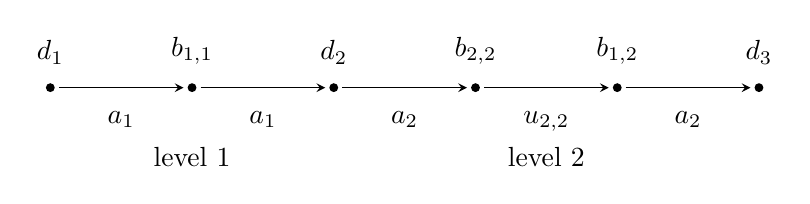
\begin{tikzpicture}[x=0.9cm,y=0.8cm,>=stealth]
 \foreach \x/\name in {0/d_1,2/b_{1,1},4/d_2,6/b_{2,2},8/b_{1,2},10/d_3}
   {\fill (\x,0) circle (1.6pt);\node[above=5pt] at (\x,0) {$\name$};}
 \draw[->] (0.12,0)--node[below=5pt] {$a_1$}(1.88,0);
 \draw[->] (2.12,0)--node[below=5pt] {$a_1$}(3.88,0);
 \draw[->] (4.12,0)--node[below=5pt] {$a_2$}(5.88,0);
 \draw[->] (6.12,0)--node[below=5pt] {$u_{2,2}$}(7.88,0);
 \draw[->] (8.12,0)--node[below=5pt] {$a_2$}(9.88,0);
 \node at (2,-1.1) {level $1$};
 \node at (7,-1.1) {level $2$};
\end{tikzpicture}
\caption{The gap coefficients for $D=3$.  The horizontal order is time
order, drawn schematically; phase order is
$b_{2,2},b_{1,1},b_{1,2}$.  Vanishing bridge totals equate the two
end coefficients on each level.}
\label{tri:gap-figure}
\end{figure}

We spell out the pairing calculation underlying the recurrence.
For $p=b_{j,i}-d_i$, its values on the same-level bridges are $2$
before $b_{j,i}$, $1$ at $b_{j,i}$, and $0$ after it.  On bridges
of a neighboring level its values are $-1$ before this phase and
$0$ after it.  Its anchor values are $1$ at $d_i$, $-1$ at
$d_{i+1}$, and zero elsewhere.
Evaluate these values on successive differences.
The contribution on its own level is minus the two gaps adjacent to
$b_{j,i}$: the additional contributions from the two end gaps cancel
because their coefficients agree.  On level $i-1$ the same endpoint
cancellation leaves the coefficient of the gap containing the phase
of $b_{j,i}$; on level $i+1$ that coefficient is obtained directly.
The contribution of the initial $d_1$ is $\boldsymbol1_{i=1}$.
With nonexistent terms interpreted as zero, this gives
\begin{equation}\label{tri:gap-pairing}
\begin{split}
 \xi_{j,i}={}&\boldsymbol1_{i=1}-u_{j,i}
 -\begin{cases}u_{j+1,i},&j<i,\\a_i,&j=i,\end{cases}\\
 &+\begin{cases}u_{j,i-1},&j<i,\\a_{j-1},&j=i,\end{cases}
 +u_{j+1,i+1}.
\end{split}
\end{equation}
Indeed the upper neighboring gap follows the event in row $j+1$;
the lower neighboring gap follows the event in row $j$ when $j<i$,
and is its initial gap when $j=i$.

Set
\[
 T_{j,i}=u_{j,i}-u_{j+1,i+1},\qquad 1\leq j\leq i\leq n_0,
\]
again using zero for nonexistent terms.  Equation~\eqref{tri:gap-pairing}
is equivalently
\begin{equation}\label{tri:gap-recurrence}
 \begin{aligned}
 T_{j,j}&=\boldsymbol1_{j=1}+a_{j-1}-a_j-\xi_{j,j},\\
 T_{j,i}&=T_{j,i-1}-\xi_{j,i} &&(i>j).
 \end{aligned}
\end{equation}
Each row of $T$ is weakly decreasing and ends in
$T_{j,n_0}=u_{j,n_0}\geq0$.  Hence every $T_{j,i}\geq0$.
The row-start inequalities then give $a_1\leq1$ and
$a_j\leq a_{j-1}$ for $j>1$.  Integrality shows that
\[
 a_1,\ldots,a_{n_0}=\underbrace{1,\ldots,1}_{e},0,\ldots,0
\]
for some $0\leq e\leq n_0$.
The case $e=n_0$ is impossible: every row-start upper bound in
Equation~\eqref{tri:gap-recurrence} would be zero, giving $T=0$
and then $u=0$, contrary to $a_1=1$.

All rows of $T$ except row $e+1$ have zero row-start upper bound.
Row $e+1$ has upper bound $1$, so its nonzero entries form an
initial stretch of ones in columns $e+1,\ldots,t$, for some
$e\leq t\leq n_0$; $t=e$ denotes an empty stretch.
The definition of $T$ telescopes along southeast diagonals:
\begin{equation}\label{tri:diagonal-recovery}
 u_{j,i}=\sum_{a\geq0}T_{j+a,i+a}.
\end{equation}
In particular $u_{1,i}=a_i$ is $1$ exactly for $1\leq i\leq t-e$.
Comparison with its already known run of length $e$ gives
$t=2e$.  Thus every positive gap coefficient is on a level
$i\leq2e$.  From~\eqref{tri:gap-recurrence}, a positive $\xi_{j,i}$
can occur only at the drop after this stretch, in level $2e+1$
(if that level exists).  In particular all $\xi_{j,i}$ on a
positively used level are zero.  When $e=0$, every gap coefficient is
zero and the possible positive value is the initial term $\xi_{1,1}$;
thus the same conclusion includes the empty stretch.

Every positively used forward root therefore pairs trivially with
$m$.  For an interior gap its pairing is the difference of the
two adjacent $\xi$ values; for the first gap it is $\xi_{i,i}$.
For the last gap it is
\[
 \Omega(d_{i+1}-b_{1,i},m)
   =\Omega(\delta_i,m)-\xi_{1,i}=0,
\]
since $K=0$ gives $\Omega(\delta_i,m)=0$ by
Equation~\eqref{tri:concavity}.  This verifies both end gaps as well
as the interior ones.

A wall increment capable of changing $[X_m]$ lies in the finite
interval $0<r\leq m-d_1$.  As $C$ is free, such an $r$ can use
only positively used gaps, and hence $\Omega(r,m)=0$.
Conjugation on that ray fixes every possible predecessor of $m$.
It follows that transport from the all-negative chamber to the
incoming direction does not change this coefficient, so
$A_m(U)=[X_m]U$.
The only vertex exponent consistent with
Lemma~\ref{tri:stationary} is $d_1$: bridges have nonzero level
total, and a pure unit vector is dominant only at the first anchor.
Therefore the only nonzero incoming coefficient of $U$ is
$A_{d_1}(U)=1$.  The definition of the incoming basis proves
$U=\Theta_{d_1}$.
\end{proof}

\subsection{Positive domination and the monomial identity}

\begin{lemma}[Vertex support before subtraction]\label{tri:domination}
For every partition $\mu\vdash N$ with at most $D$ parts, padded by
zeroes, put $x_\mu=\sum_i\mu_i d_i$.  In the all-negative chamber,
$\Theta_{x_\mu}$ has nonnegative vertex exponents and coefficients
in $\N[v,v^{-1}]$, and is a finite Laurent polynomial.  More
precisely, coefficientwise in both vertex exponents and $v$,
\begin{equation}\label{tri:positive-domination}
 \frac{N!}{\prod_i\mu_i!}\,\Theta_{x_\mu}\ \leq\ U^N.
\end{equation}
\end{lemma}

\begin{proof}
Lemma~\ref{tri:linear} and Corollary~\ref{wall:product} give a
nonnegative incoming expansion of $U^N$.
Lemma~\ref{tri:pure}, applied to $(z_1+\cdots+z_D)^N$, gives
\[
 A_{x_\mu}(U^N)=\frac{N!}{\prod_i\mu_i!}>0.
\]
Every section in this expansion has nonnegative coefficients in
every chamber by Theorem~\ref{wall:positivity}.  Retaining the one
displayed summand therefore gives~\eqref{tri:positive-domination}.
The right side is a finite Laurent polynomial with nonnegative
vertex exponents and nonnegative integral coefficients in $v$.
No coefficient outside that finite support, and no negative
vertex coordinate, can occur in the retained positive summand.
This proves all the claims, including finiteness of its Laurent
coefficients.  The case $N=0$ is the identity section.
\end{proof}

\begin{theorem}[Monomial sections]\label{tri:monomial}
For every partition $\lambda$ with at most $D$ parts, padded by
zeroes to length $D$, one has in the all-negative chamber
\begin{equation}\label{tri:monomial-identity}
 m_\lambda(Y)=\Theta_{\sum_{i=1}^D\lambda_i d_i}.
\end{equation}
In particular,
\begin{equation}\label{tri:elementary-identity}
 E_k=\Theta_{d_1+\cdots+d_k}\qquad(0\leq k\leq D).
\end{equation}
\end{theorem}

\begin{proof}
For $D=1$ the cone is trivial and the assertion is immediate.
Otherwise set $N=|\lambda|$ and $x_\lambda=\sum_i\lambda_i d_i$.
The polynomial $m_\lambda(Y)$ has nonnegative vertex exponents:
it is a polynomial in the independent-set generators, each of
which has this support property.  This assertion concerns its
exponent support and does not assume coefficient positivity.
Lemma~\ref{tri:domination} already gives the same support property
for $\Theta_{x_\lambda}$.

By Lemmas~\ref{tri:stationary} and~\ref{tri:pure}, the pure
incoming coefficients of $m_\lambda(Y)$ are $1$ at $x_\lambda$
and zero at every other pure label.  Indeed $m_\lambda$ is the
sum of the distinct ordinary monomials in the orbit of $\lambda$,
and that orbit contains exactly one dominant vector.
Subtract the indicated section and write
\[
 F=m_\lambda(Y)-\Theta_{x_\lambda}.
\]
Its ordinary support still has nonnegative vertex coordinates,
all its pure incoming coefficients vanish, and both its ordinary
and incoming support lie in $Nd_1+C^+$.

If an incoming coefficient remains nonzero, its label $m$ is
mixed and satisfies $K_i(m)=0$ by Lemma~\ref{tri:stationary};
subtracting $\Theta_{x_\lambda}$ changes only one pure incoming
coefficient.  A nonzero bridge-coordinate vector with zero sum
on each level has some negative bridge coordinate.
Among all remaining labels choose one with minimum height in
$Nd_1+C^+$, where the height is the sum of its nonnegative simple
root coordinates.  A minimum exists in $\N$, even if the incoming
expansion is infinite.  Incoming triangularity says that the
ordinary coefficient at this label equals its incoming
coefficient plus contributions from strictly lower incoming
labels.  There are no such nonzero lower terms by the choice of
height.  Hence $[X_m]F=A_m(F)\ne0$, contradicting the negative
bridge coordinate of $m$ and the vertex support already proved.
No coefficient remains, proving~\eqref{tri:monomial-identity}.
Finally $m_{(1^k)}=e_k$ gives~\eqref{tri:elementary-identity}.
\end{proof}


\begin{corollary}[Elementary positivity]\label{tri:positivity}
Let $G$ be a natural unit interval graph on $n$ vertices, and put
$M=|E(G)|$.  In its elementary expansion
\[
 \chi_G(X;q)=\sum_{\lambda\vdash n}c_\lambda(q)e_\lambda(X),
\]
every $c_\lambda(q)$ belongs to $\N[q]$ and has degree at most $M$.
For a triangular embedding with $D\geq n$, let $u$ be the sum of the
selected vertex exponents and set $x_\lambda=\sum_i\lambda_i d_i$,
padding $\lambda$ by zeroes.  Then
\begin{equation}\label{tri:positive-coefficient}
 [X_u]\Theta_{x_\lambda}^{H_-}
   =v^{-M}c_\lambda(v^2)
   \in\sum_{d=0}^{M}\N v^{2d-M},
\end{equation}
where $H_-$ is the all-negative chamber.
\end{corollary}

\begin{proof}
Choose the embedding of Lemma~\ref{tri:embedding}, taking $D\geq n$.
Proposition~\ref{graph:kernel}, Lemma~\ref{graph:reciprocity}, and
Theorem~\ref{tri:monomial} give
\[
 c_\lambda(v^2)=v^M[X_u]m_\lambda(Y)
              =v^M[X_u]\Theta_{x_\lambda}^{H_-}.
\]
The last expression has nonnegative integral coefficients at every
power of $v$ by Theorem~\ref{wall:positivity}.
On the other hand, the coloring definition has $q$-degree at most
$M$.  In any number of variables at least $n$, the elementary
monomials form an integral basis in degree $n$; symmetry therefore
gives $c_\lambda(q)\in\Z[q]$ of degree at most $M$.
Comparing these finite polynomials with the displayed Laurent-series
identity proves coefficientwise nonnegativity and
Equation~\eqref{tri:positive-coefficient}.
\end{proof}

This completes the coefficientwise positivity assertion.  The remaining
construction assigns a partition to each individual graph-nondescent
permutation and proves the weight-preserving formula in
Theorem~\ref{main:theorem}.  The finite coefficient bounds in
Equation~\eqref{tri:positive-coefficient} will also bound the histories
used by that construction.

\section{A finite witness on individual words}
\label{route:section}

Corollary~\ref{tri:positivity} proves positivity of the elementary
coefficients. We now construct the partition assigned to each individual
word. The construction matches ordered packets of vertices with finite
wall histories and anchor words; the anchor multiplicities specify the
partition. Its local matchings use coefficients of elementary sections
and individual wall operators, without taking the final elementary
coefficient list as input.

Fix a triangular embedding with $D\geq\max\{1,n\}$, put $N=n$, and
let $u$ be the sum of the indicated vertex exponents.  Write $H_-$ for its all-negative chamber,
$M=|E(G)|$, and
\[
 R=u-Nd_1\in C^+,
 \qquad B=\{y:Nd_1\leq y\leq u\}.
\]
The order in this display is the free-cone order.  If
$R=\sum_{c\in C}R_c c$, set $h(R)=\sum_c R_c$.
The set $B$ has $\prod_c(R_c+1)$ elements.  Only wall roots $0<r\leq R$
can contribute to the coefficients considered here.  All chamber and
path choices in this section refer to this finite truncation.

\subsection{Decorated coefficients and their finite orders}
\label{route:decorations}

For $1\leq k\leq N$, let
\[
 E_k=e_k(Y)=\Theta_{d_1+\cdots+d_k},
 \qquad E_k^H=\sum_{a,e}c_k^H(a,e)v^eX_a.
\]
The identity is Theorem~\ref{tri:monomial}.  The coefficients
$c_k^H(a,e)$ are nonnegative integers by Theorem~\ref{wall:positivity}.
A decorated $k$-packet in $H$ is a triple $(a,e,t)$ with
$1\leq t\leq c_k^H(a,e)$.  The integer $e$ is its energy.  For an ordered
composition ${\boldsymbol k}=(k_1,\ldots,k_b)$ of $N$, a product state is
an ordered tuple of decorated packets.  Its exponent and energy are
\begin{equation}
 \label{route:product-energy}
 a=\sum_{i=1}^b a_i,
 \qquad
 E=\sum_{i=1}^b e_i+\sum_{i<j}\Omega(a_i,a_j).
\end{equation}
Thus these states count the coefficients of $P_{\boldsymbol k}
=E_{k_1}\cdots E_{k_b}$, with their multiplicities.  In $H_-$, a packet
is just an independent set of size $k$, with energy zero and index one.

If a wall operator $W$ is positive on $X_a$, a decorated jump from $a$
to $a+jp$ is a triple $(j,e,t)$ with
\begin{equation}
 \label{route:jump-decoration}
 j\geq0,\qquad
 1\leq t\leq [v^eX_{a+jp}]W(X_a).
\end{equation}
Here $p$ is the primitive positive lattice vector of the wall ray; an
unoccupied multiple simply has coefficient zero.  Energies in
Equation~\eqref{route:jump-decoration} are in centered torus notation and already
include the shift arising from multiplication by $X_a$.  The unique
zero jump is $(0,0,1)$.

\begin{lemma}[Effective coefficient slices]
\label{route:finite}
At fixed total exponent in $B$ and fixed total energy, every packet
decomposition and local jump decomposition used below is a finite set
that can be enumerated effectively.  The same holds for a sequence of at most
$h(R)$ nonzero total jumps.
\end{lemma}

\begin{proof}
The support of $E_k$ in every chamber is contained in $kd_1+C^+$.
Consequently every packet offset and every jump increment in a
decomposition with total exponent at most $u$ is at most $R$.
There are finitely many exponent tuples, wall directions, and truncated
chambers.  This assertion applies to underlying packet states as well
as to their states after jumps.

At each fixed exponent the coefficient of a section or wall jump lies
in $\Z((v^{-1}))$: it has a finite upper energy bound and finite
coefficients at individual energies.  For a fixed exponent tuple,
write its energy equation as
\[
 E=\kappa+e_1+\cdots+e_s,
\]
where $\kappa$ is the fixed sum of torus cross terms.  If the coefficient
of the $i$th piece has upper energy bound $U_i$, then
\begin{equation}
 \label{route:energy-bound}
 E-\kappa-\sum_{j\ne i}U_j\ \leq e_i\leq U_i.
\end{equation}
Thus each energy and each decoration ranges over a finite set.  For
bounded sequences there are again only finitely many exponent types,
so the same argument applies to all their pieces at once.

These are effective bounds.  The initial units have the rational
coefficients
\[
 [X_{jp}]D_p=
 \frac{v^{-j^2}}{\prod_{i=1}^j(1-v^{-2i})}.
\]
The triangular factorization and incoming equations of
Section~\ref{wall:section} determine every wall coefficient to the
required root order by finite rational arithmetic in $v$.  Transport
of the finite independent-set sums determines the needed $E_k^H$ in
the same way.  A rational function expanded at $v^{-1}=0$ has a
computable upper degree, and any finite interval of its coefficients
is computable by formal division.  Reducing numerator and denominator
first also decides whether it vanishes.  One may therefore compute
the bounds in Equation~\eqref{route:energy-bound}, enumerate all choices in
them, and compute their multiplicities.  No factorization into
positive units needs to be found in order to perform these
coefficient calculations; positivity justifies interpreting the
computed integers as multiplicities.
\end{proof}

We specify the finite choices used by these definitions. Order lattice
coordinates in the basis $d_1$, followed by the forward roots $C$ in
time order and then any added dual basis vectors.
For a nonnegative integer $a$,
let $b(a)$ be its binary expansion, with $b(0)=0$, and encode it as
$1^{|b(a)|}0b(a)$.  Encode a signed integer by a sign bit followed by
the code of its absolute value, a rational by its reduced numerator
and positive denominator, and a tuple by its length followed by its
component codes.  A fixed initial type tag distinguishes these
possibilities.  Sign vectors are tuples of signed integers.  Order
codes first by length and then lexicographically.  In every finite
set below, ``the same index'' means the same rank in this order.
Fix the triangular embedding by the same order: enumerate tuples giving
an integer $D\geq\max\{1,n\}$, rational phases in the order of
Equation~\eqref{tri:phase-order}, and $n$ distinct selected bridges,
and take the first tuple whose induced ordered graph is $G$.
Every candidate is checked by finitely many rational comparisons, and
Lemma~\ref{tri:embedding} proves that a candidate exists.  For empty
input use $D=1$ and no selected bridges.

All later generic rational choices mean the first code satisfying the
listed open inequalities and avoidance conditions.  These are decidable
finite systems of rational linear conditions.  In particular, for a
line $h+tV(y)$, two distinct wall hyperplanes with nonzero pairings
have simultaneous crossings precisely when
$h(r)\Omega(s,y)-h(s)\Omega(r,y)=0$.  A root $r$ with
$\Omega(r,y)=0$ instead requires $h(r)\ne0$.  Thus the path conditions
used below have the asserted finite form.  A nonempty open rational cell contains a rational
point, so the searches terminate.

\subsection{The local packet switch}
\label{route:local}

Let $W:I\longrightarrow II$ be a wall crossing on the positive ray
$\N p$.  Write its operator as $\operatorname{Ad}(g_p)^\varepsilon$,
where $\varepsilon=1$ for a crossing from positive to negative and
$\varepsilon=-1$ for the reverse crossing.  Assume that the target
exponent $y$ satisfies
\begin{equation}
 \label{route:positive-total}
 \varepsilon\Omega(p,y)\geq0.
\end{equation}
This is exactly the positive bend direction of
Proposition~\ref{wall:factors}, with the identity direction included
as in Lemma~\ref{wall:unit}.

The total pairing in Equation~\eqref{route:positive-total} can be
nonnegative even when an individual packet has negative pairing.
The switch must therefore use both directions of single-packet
transport. Its invariant is a tuple of packet states retained on
the side from which their jumps have nonnegative coefficients.

\begin{proposition}[Packet switch]
\label{route:switch}
There is a computable energy-preserving bijection
\begin{equation}
 \label{route:switch-equation}
 \left\{\text{product states of exponent $y$ in $II$}\right\}
 \longleftrightarrow
 \left\{\begin{array}{c}
  \text{product states of exponent $z$ in $I$, together with}\\
  \text{a decorated jump of $W$ from $z$ to $y$}
 \end{array}\right\}.
\end{equation}
On the right the energy is the state energy plus the jump energy.
If $\Omega(p,y)=0$, the total jump is always the unique zero jump.
\end{proposition}

\begin{proof}
For a packet with exponent $a$, call its type positive if
$\varepsilon\Omega(p,a)\geq0$, and negative otherwise.  Adding a
multiple of $p$ does not change this type.  In particular the types
are recoverable on both sides of Equation~\eqref{route:switch-equation}.

For a positive packet the section identity $E_k^{II}=W(E_k^I)$
expresses each decorated state in $II$ as a state in $I$ followed by
a positive jump of $W$.  More precisely, at fixed output exponent
and energy the two sets have the same cardinality, so identify them
by their finite ranks from Lemma~\ref{route:finite}.  For a negative
packet use instead $E_k^I=W^{-1}(E_k^{II})$: a state in $I$ is
identified with a state in $II$ followed by a positive jump of
$W^{-1}$.  Packets of zero pairing are fixed.  These identifications
have computable inverses.

Fix the retained state of each packet: in chamber $I$ for a positive
packet, and in chamber $II$ for a negative packet. Write $x_i$ for
its exponent, and keep its energy and decoration index fixed.
The two positive expansions to be matched are
\[
\begin{array}{c|c|c|c}
\text{packet type}&\text{retained chamber}&
 L_i\ \text{(side $II$)}&R_i\ \text{(side $I$)}\\ \hline
\text{positive}&I&W(X_{x_i})&X_{x_i}\\
\text{negative}&II&X_{x_i}&W^{-1}(X_{x_i})
\end{array}
\]
Via the single-packet bijections, a decorated term of $L_i$ together
with its retained state gives a packet in $II$; a decorated term of
$R_i$ together with that state gives a packet in $I$.
Each row satisfies $L_i=W(R_i)$, so the automorphism property gives
\begin{equation}
 \label{route:automorphism}
 L_1\cdots L_b=W(R_1\cdots R_b).
\end{equation}
The left side opens only positive packets. The right side opens only
negative packets and then applies one total jump. For a term at
$X_y$, the input of the total jump differs from $y$ by a multiple
of $p$. Its pairing is therefore $\Omega(p,y)$, and
Equation~\eqref{route:positive-total} makes that jump positive.

We spell out the energy in Equation~\eqref{route:automorphism}.  If the
individual increments in a term are $j_i p$, its cross-packet shift is
\begin{equation}
 \label{route:cross-energy}
 \begin{split}
 \sum_{i<j}\Omega(x_i+j_i p,x_j+j_j p)
 ={}&\sum_{i<j}\Omega(x_i,x_j)\\
 &+\sum_{i<j}\bigl(j_i\Omega(p,x_j)
                         +j_j\Omega(x_i,p)\bigr).
 \end{split}
\end{equation}
There is no quadratic term because $\Omega(p,p)=0$.  On the right
of Equation~\eqref{route:automorphism}, add the energy of the final total
jump to this expression and to the individual inverse-jump energies.
On the left, add the individual forward-jump energies.  Taking a
fixed $v$-coefficient of $X_y$ in the identity gives equality of the
two finite sets of jump tuples with exactly these energies.
Match them by rank.  Restoring the fixed underlying packet energies
adds the same integer to both sides.

The bijection is now explicit in either direction.  From the left of
Equation~\eqref{route:switch-equation}, open its positive packets by their
single-packet bijections, keep its negative packets as underlying
states, apply the jump-tuple rank bijection, and close the negative
packets into states in $I$.  Conversely, from the right, open the
negative packets, retain the positive packets, invert the jump-tuple
bijection, and close the positive packets into states in $II$.
Invariant packet types ensure that the same underlying data and rank
sets are used on reversal.  All ranks are finite by
Lemma~\ref{route:finite}.  Finally, if $\Omega(p,y)=0$, every monomial
on the line $y+\Z p$ commutes with $g_p$, so its total transform has
only the zero jump.
\end{proof}

\begin{example}[Zero total jump with changing packets]
\label{route:zero-example}
In the monomial identity of the switch, take $W=\Ad(D_p)$ and
$\Omega(p,x_1)=1$, $\Omega(p,x_2)=-1$.
The two sides of Equation~\eqref{route:automorphism} become
\[
 (X_{x_1}+X_{x_1+p})X_{x_2}
   =X_{x_1}(X_{x_2}+X_{x_2+p}).
\]
The total pairing is zero, so $W$ fixes every monomial in the
right-hand product. The terms at exponent $x_1+x_2+p$ agree because
\[
 \Omega(x_1+p,x_2)=\Omega(x_1,x_2+p)=\Omega(x_1,x_2)-1.
\]
Thus the local matching transfers the increment from the positive
packet to the negative packet while its recorded total jump is zero.
The example concerns the monomial matching with retained exponents
fixed; its point is that zero total jump need not fix each packet.
\end{example}

\subsection{Common histories and terminal anchor states}
\label{route:histories}

Before choosing a composition, fix a generic rational representative
$h_{H,y}\in H$ for every truncated chamber $H$ and every $y\in B$.
Use the line $h_{H,y}+tV(y)$, $t\geq0$.  Choose the representatives
so that its transverse wall crossings are distinct and avoid joints.
There are only finitely many avoidance conditions.  At large $t$ it
lies in a testing chamber near $V(y)$; if $V(y)=0$, the line is
constant and has no crossings.  List its crossings in the direction
of decreasing $t$, toward $H$.  Each has the sign required by
Equation~\eqref{route:positive-total}.  The choices depend on $(H,y)$ only,
not on the number, sizes, energies, or indices of packets.

For a section $P$ supported above $Nd_1$, the coefficient recursion
of Lemma~\ref{wall:recursion} is
\begin{equation}
 \label{route:history-recursion}
 [X_y]P^H=A_y(P)+
 \sum_{W:I\to II}\ \sum_{Nd_1\leq z<y}
       [X_y]W(X_z)\,[X_z]P^I.
\end{equation}
The outer sum follows the selected line, oriented toward $H$.
Only increments on the crossed ray have nonzero coefficients.
The zero-jump coefficient is one, which is why
Equation~\eqref{route:history-recursion} is a sum of increments rather than
a product of separate wall choices.

Define a total history from $(H_-,u)$ recursively.  At a pair $(H,y)$
it either stops, with terminal label $y$, or chooses one crossing
$W:I\to II$ in Equation~\eqref{route:history-recursion}, an exponent $z<y$,
and a nonzero decorated jump from $z$ to $y$, then continues from
$(I,z)$.  Its energy is the sum of its jump energies.  Let $T_x$ be
the set of histories with terminal label $x$, and $T_x(E)$ its energy
$E$ slice.  The choices of crossing and chamber at each step are
part of the history, so equal-looking jumps on different portions
of a path are distinguished.

Every nonzero jump lowers the cone height by at least one, so a
history has at most $h(R)$ such jumps.  Lemma~\ref{route:finite}
proves directly that $T_x(E)$ is finite.  Applying
Equation~\eqref{route:history-recursion} to $\Theta_x$, whose incoming
coordinates are $A_y(\Theta_x)=\mathbf1_{y=x}$, gives
\begin{equation}
 \label{route:history-series}
 \sum_{t\in T_x}v^{E(t)}=[X_u]\Theta_x^{H_-}.
\end{equation}
This is a coefficientwise identity in the Laurent completion.
The definition of $T_x$ itself uses only local monomial jumps.

The packet realization of this recursion is also reversible.  Start
with a product state of exponent $y$ in $H$, and traverse the chosen
line backwards, applying Proposition~\ref{route:switch} at each
wall.  A zero total jump continues to the next wall.  At the first
nonzero total jump, record its crossing and decoration and recurse
from the smaller exponent and its chamber.  If every total jump is
zero, stop with the product state in the testing chamber.  Between
two nonzero jumps only finitely many walls are crossed.  For the
inverse, first reconstruct the state in $(I,z)$ recursively.  Apply
the inverse local switch with the recorded jump $z\to y$ to obtain
its state in chamber II, then undo the zero-jump switches between
II and $H$.  At a stopping leaf, begin with its terminal testing
state and undo every zero-jump switch on that selected line.
Thus for every composition this procedure is a
bijection to histories with their terminal product states.  It uses
literally the same $T_x$ for all compositions.

\begin{lemma}[Return to the anchors]
\label{route:return}
A nonempty terminal product state has label
$x=x_\mu=\sum_{i=1}^D\mu_i d_i$ for a partition $\mu\vdash N$,
padded by zeroes.  Keeping its total history fixed, it can be
transported bijectively to an ordered tuple of anchor subsets of
sizes $k_1,\ldots,k_b$ and total exponent $x_\mu$.  Every such
anchor tuple has energy zero.
\end{lemma}

\begin{proof}
In ordinary commuting variables $z_1,\ldots,z_D$, expand
\begin{equation}
 \label{route:anchor-product}
 \prod_{j=1}^b e_{k_j}(z)=\sum_{\mu\vdash N}a_{\boldsymbol k,\mu}
 m_\mu(z).
\end{equation}
The nonnegative integer $a_{\boldsymbol k,\mu}$ is the number of
ordered subsets of $[D]$ of the specified sizes in which index $i$
occurs $\mu_i$ times.  By Theorem~\ref{tri:monomial}, the incoming
coordinates of $P_{\boldsymbol k}$ are exactly these constants at
$x_\mu$ and zero elsewhere.  A testing-chamber state therefore has
one of these labels, and its total coefficient there is the
constant $a_{\boldsymbol k,\mu}$.

The coefficient at the same pure label in $H_-$ is also
$a_{\boldsymbol k,\mu}$.  Indeed the initial independent-set
monomials have nonnegative vertex coordinates, so a tuple using a
bridge cannot contribute to an exponent with every bridge
coordinate zero.  All remaining tuples use anchors, which are
mutually independent and pair by zero.  Their packet energies and
cross-packet shifts are zero.

Here is a transport of the states, rather than just an equality of
their number.  Fix a generic all-negative rational covector $h_-$.
Within a sufficiently small neighborhood of the testing direction
$V(x)$, move the terminal chamber to the chamber of
$h_-+tV(x)$ for large $t$.  Only hyperplanes with
$\Omega(p,x)=0$ can separate these two perturbations.  Their
packet switches have zero total jump by
Proposition~\ref{route:switch}.  Next follow $h_-+tV(x)$ down to
$t=0$.  Every crossed positive root $p$ has
$\Omega(p,x)>0$, and the crossing is from positive to negative.
At each crossing, the coefficient of $X_x$ gains only nonnegative
contributions from lower exponents, with its old coefficient
retained by the zero jump.  Its starting and ending coefficients
are the same constant $a_{\boldsymbol k,\mu}$.  Coefficientwise
positivity forces every gain along this finite path to be zero.

It follows that, in Equation~\eqref{route:switch-equation} for these product
states at $x$, only the zero-total-jump part occurs at every wall.
The switches consequently give bijections all the way to the
literal anchor tuples in $H_-$.  Reversing the selected path gives
the inverse.  All intermediate choices can be fixed by the rational
ordering above; they may use the composition but add no total jump
to the recorded history.  The history determines its terminal
testing chamber, so the inverse loses no data.
\end{proof}

\begin{proposition}[Formal degree bounds]
\label{route:parity}
For every partition $\mu\vdash N$, histories in $T_{x_\mu}$ have
\begin{equation}
 \label{route:parity-range}
 -M\leq E(t)\leq M,\qquad E(t)\equiv M\pmod 2.
\end{equation}
Consequently $T_{x_\mu}$ is finite, and
$v^M[X_u]\Theta_{x_\mu}^{H_-}$ belongs to $\N[q]$ with $q=v^2$
and degree at most $M$.
\end{proposition}

\begin{proof}
Equation~\eqref{route:history-series} identifies the history enumerator
with $[X_u]\Theta_{x_\mu}^{H_-}$. By
Equation~\eqref{tri:positive-coefficient}, this coefficient is
$v^{-M}c_\mu(v^2)$, where $c_\mu(q)\in\N[q]$ has degree at most $M$.
Its allowed powers of $v$ are therefore exactly among
$-M,-M+2,\ldots,M$. Histories have nonnegative multiplicities, so
none can occur at any other energy. Each of these finitely many
energy slices is finite by Lemma~\ref{route:finite}; hence their
union $T_{x_\mu}$ is finite as well. Multiplication by $v^M$ changes
each history weight to $q^{(E(t)+M)/2}$, proving the assertion.
\end{proof}

\subsection{Required masks and exact masks}
\label{route:masks}

For a permutation word $w=w_1\cdots w_N$ on the indicated vertices,
define its nonedge ascent mask by
\[
 \mathcal P_G(w)=
 \{j: w_j<w_{j+1},\ \{w_j,w_{j+1}\}\notin E(G)\}.
\]
For a word $s=s_1\cdots s_N$ on the labeled anchor indices
$[D]$, define its ascent mask by
$\mathcal Q(s)=\{j:s_j<s_{j+1}\}$.
For a subset $J\subseteq[N-1]$, a \emph{required} mask means
$J\subseteq\mathcal P_G(w)$ or $J\subseteq\mathcal Q(s)$;
an \emph{exact} mask means equality.  These are different conditions.

Place packet boundaries exactly at the complement of $J$.  This
gives a composition ${\boldsymbol k}(J)$ of $N$.  If
$J\subseteq\mathcal P_G(w)$, each packet is an increasing independent
set.  In fact, if successive letters $a<b$ in a packet satisfy
$h(a)<b$, then every later letter $c\geq b$ also satisfies
$h(a)<c$.  Hence every pair in that packet is a nonedge.
Conversely, an independent set in increasing order has precisely
the required internal ascents.  Product states at $u$ for this
composition are therefore exactly the words with the required
mask $J$.  Their energies are
\begin{equation}
 \label{route:word-energy}
 E(w)=2\inv_G(w)-M,
\end{equation}
since no edge is internal to a packet and
Equation~\eqref{route:product-energy} counts every edge between packets.

At a terminal label $x_\mu$, writing each anchor subset in increasing
index order gives a word with multiplicities
$(\mu_1,\ldots,\mu_D)$ and with $J\subseteq\mathcal Q(s)$.
Lemma~\ref{route:return} and the history construction therefore give
a computable bijection, with computable inverse,
\begin{equation}
 \label{route:required-bijection}
 B_J:\{w:J\subseteq\mathcal P_G(w)\}
 \longrightarrow
 \coprod_{\mu\vdash N}
 \{(t,s):t\in T_{x_\mu},\
       \operatorname{mult}(s)=\mu,\ J\subseteq\mathcal Q(s)\}.
\end{equation}
It satisfies $E(t)=E(w)$.  The target histories in this formula are
the same for every $J$; only the permitted words $s$ change.

We convert the required-mask bijections to exact-mask bijections by
finite bijective cancellation, in the spirit of the Garsia--Milne
involution principle \cite{GM81}.  The complete alternating-path
argument below also supplies termination in both directions.

\begin{lemma}[Exact-mask refinement]
\label{route:exact}
For every $J\subseteq[N-1]$ there is a computable energy-preserving
bijection $\Phi_J$ between the two sides of
Equation~\eqref{route:required-bijection} with their masks required to be
\emph{exactly} $J$.  Both directions terminate on every input.
\end{lemma}

\begin{proof}
Construct the bijections in decreasing order of $|J|$, breaking ties
by the fixed subset order.  For an exact-$J$ input $w$, apply $B_J$.
If its output $(t,s)$ has exact mask $J$, stop.  Otherwise put
$K=\mathcal Q(s)\supsetneq J$, apply the already constructed inverse
$\Phi_K^{-1}$, and apply $B_J$ again.  Repeat this instruction.
For the inverse procedure start at an exact-$J$ pair, apply
$B_J^{-1}$, and, whenever the resulting word has exact mask
$K\supsetneq J$, apply $\Phi_K$ followed by $B_J^{-1}$.
Thus every nested call involves a strictly larger mask.

To prove that the outer repetition terminates, fix its energy $E$.
The required-$J$ source is finite, and its target is finite by
Lemma~\ref{route:finite} (also by
Proposition~\ref{route:parity}).  On their disjoint union draw the
matching given by $B_J$.  On the vertices whose exact masks strictly
contain $J$, draw a second matching, the disjoint union of the
already defined $\Phi_K$ for $K\supsetneq J$.  Each vertex has one
edge of the first matching, and either zero or one edge of the
second.  Distinct edges that happen to have the same endpoints are
retained as distinct matching edges.
Figure~\ref{route:matching-figure} illustrates the alternating path in
their union.

An exact-$J$ starting vertex is an endpoint of this finite graph.
Its component is a path, not a cycle: all vertices have degree at
most two, and a component containing a degree-one vertex cannot be
a cycle.  Following its alternating edges therefore never revisits
a vertex and eventually reaches the other endpoint.  A return edge
of the second matching always lands at a source with a larger
exact mask, where the first matching can be followed again.
Consequently the other endpoint lies on the target side and has
exact mask $J$.  Reversing the same path is precisely the inverse
procedure described above.  Every edge preserves $E$, proving the
claimed energy preservation as well as termination.
\end{proof}

\begin{figure}[htbp]
\centering
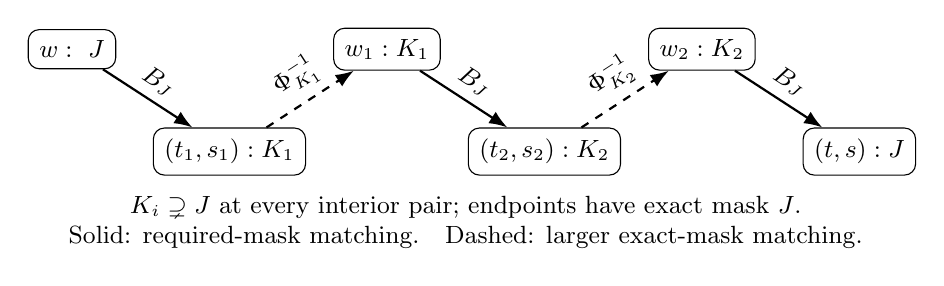
\begin{tikzpicture}[>=Latex,
  vertex/.style={draw,rounded corners,inner sep=4pt,font=\small}]
 \node[vertex] (l0) at (0,1.3) {$w:\ J$};
 \node[vertex] (r1) at (2,0) {$(t_1,s_1):K_1$};
 \node[vertex] (l1) at (4,1.3) {$w_1:K_1$};
 \node[vertex] (r2) at (6,0) {$(t_2,s_2):K_2$};
 \node[vertex] (l2) at (8,1.3) {$w_2:K_2$};
 \node[vertex] (r0) at (10,0) {$(t,s):J$};
 \draw[->,thick] (l0)--node[above,sloped,font=\small] {$B_J$} (r1);
 \draw[->,thick,dashed] (r1)--node[above,sloped,font=\small]
   {$\Phi_{K_1}^{-1}$} (l1);
 \draw[->,thick] (l1)--node[above,sloped,font=\small] {$B_J$} (r2);
 \draw[->,thick,dashed] (r2)--node[above,sloped,font=\small]
   {$\Phi_{K_2}^{-1}$} (l2);
 \draw[->,thick] (l2)--node[above,sloped,font=\small] {$B_J$} (r0);
 \node[font=\small,align=center] at (5,-0.9)
   {$K_i\supsetneq J$ at every interior pair; endpoints have exact mask $J$.\\
    Solid: required-mask matching.\quad Dashed: larger exact-mask matching.};
\end{tikzpicture}
\caption{The exact-mask algorithm follows a finite alternating path.
An endpoint cannot enter a cycle in the union of two matchings.}
\label{route:matching-figure}
\end{figure}

\subsection{The partition assigned to a word}
\label{route:algorithm}

Let $\mathcal A_G=\{w:\mathcal P_G(w)=\varnothing\}$ be the
admissible domain.  For $w\in\mathcal A_G$, compute
\[
 \Phi_{\varnothing}(w)=(t,s),\qquad t\in T_{x_\mu},
 \qquad \Lambda_G(w)=\mu.
\]
The finite algorithm on an individual input has four steps.
\begin{enumerate}
\item Construct the triangular embedding and finite cone interval, and
fix the common rational path representatives for every required $(H,y)$
before choosing any packet composition.
\item For each required mask encountered, form its packets and evaluate
$B_J$ through the local packet switches, common histories, and return
to anchor subsets. Positive and negative packets use the two directions
of the local switch, although the total jump has the positive sign.
\item Evaluate $\Phi_{\varnothing}$ by the exact-mask recursion in
Lemma~\ref{route:exact}, following its alternating walk until the output
has exact empty mask.
\item Read the multiplicities of the resulting weakly decreasing anchor
word as the partition $\Lambda_G(w)$.
\end{enumerate}
Nested calls strictly increase mask size, while each outer repetition
follows an endpoint path in the finite union of two matchings. Thus the
call depth is bounded and each alternating walk terminates. There is
no need to enumerate the final fibers of $\Lambda_G$ or to supply the
final elementary coefficients. Section~\ref{main:completion} gives the
reversal for the original input convention.
If the input is supplied in the insertion digits of
Lemma~\ref{graph:digits}, first decode those digits by largest-vertex
insertions.  The construction then uses the resulting admissible
word.  Empty input is assigned the empty partition.

\begin{theorem}[Permutation witness]
\label{route:witness}
For every naturally labeled unit interval graph $G$, the preceding
finite rule assigns a partition $\Lambda_G(w)\vdash n$ to each
$w\in\mathcal A_G$ and satisfies the formal polynomial identity
\begin{equation}
 \label{route:witness-identity}
 X_G(X;q)=\sum_{w\in\mathcal A_G}
                   q^{\inv_G(w)}e_{\Lambda_G(w)}(X).
\end{equation}
In particular, every elementary coefficient is in $\N[q]$ and has
degree at most $|E(G)|$.
\end{theorem}

\begin{proof}
For any padded partition $\mu$, exactly one word of multiplicities
$(\mu_1,\ldots,\mu_D)$ has no strict ascent: the weakly decreasing
word.  This remains true when parts of $\mu$ repeat, since the
anchor indices themselves are distinct labels.  Consequently
$\Phi_{\varnothing}$ identifies the individual words of shape
$\mu$ with $T_{x_\mu}$.  Energy preservation,
Equation~\eqref{route:word-energy}, and Equation~\eqref{route:history-series} give
\[
 \sum_{\substack{w\in\mathcal A_G\\\Lambda_G(w)=\mu}}
       v^{2\inv_G(w)-M}
   =\sum_{t\in T_{x_\mu}}v^{E(t)}
   =[X_u]\Theta_{x_\mu}^{H_-}
   =[X_u]m_\mu(Y).
\]
Multiply by $v^M$.  The conversion $q=v^2$ is legitimate as a
formal polynomial conversion by
Proposition~\ref{route:parity}, including both its parity and its
degree bounds.  The coefficient identity of
Proposition~\ref{graph:kernel} now identifies the right side with
$[e_\mu]X_G(X;q)$.  This proves the identity for each shape and
hence Equation~\eqref{route:witness-identity}. The algorithms producing
$\Lambda_G(w)$ use only elementary packets and local wall jumps;
the coefficient identity certifies their output.
\end{proof}

\section{The chromatic expansion}
\label{main:completion}

We return to the original graph and its graph-nondescent permutations.

\begin{proof}[Proof of Theorem~\ref{main:theorem}]
Choose the triangular embedding of Lemma~\ref{tri:embedding}, and
fix the rational generic choices and finite local orders in
Section~\ref{route:section} by the enumeration specified there.
Theorem~\ref{route:witness} gives a terminating map
$\Lambda_G:\mathcal A_G\to\{\lambda:\lambda\vdash n\}$ with
\[
 \sum_{\substack{w\in\mathcal A_G\\\Lambda_G(w)=\lambda}}
       q^{\inv_G(w)}
   =[e_\lambda]X_G(X;q)=c_\lambda(q).
\]
For $\sigma\in D_G^0$ define
\[
 \theta_G(\sigma)=\Lambda_G(\operatorname{reverse}\sigma).
\]
By Lemma~\ref{graph:digits}, reversal gives the required input to
$\Lambda_G$ and complements graph inversions. Lemma~\ref{graph:reciprocity}
then gives, for every $\lambda$,
\[
 \sum_{\substack{\sigma\in D_G^0\\\theta_G(\sigma)=\lambda}}
       q^{\ginv_G(\sigma)}
   =q^M c_\lambda(q^{-1})=c_\lambda(q).
\]
Together with $X_G=\chi_G$, this proves
Equation~\eqref{main:witness}. Every coefficient is the generating
polynomial of a finite set, so it belongs to $\N[q]$. All choices and
all recursions are finite procedures for each input. For $n=0$, take
the empty graph, the empty permutation and the empty partition.
\end{proof}

\begin{remark}[Scope of the algorithm]
The map uses the graph, the input permutation, finite wall recursions
and local coefficient indexings. The elementary coefficient list is
not supplied to it. The result proves termination, but gives no
polynomial-time bound. The construction is a mathematical algorithm
based on finite rational arithmetic and ordered finite sets.
\end{remark}

\clearpage
\bibliographystyle{plainnat}
\bibliography{references}
\end{document}
